\chapter{La réalisation }
\label{sec:conception}

\begin{fquote}Puisque Scrum est choisi comme méthode de gestion de projets, ce chapitre va être réparti selon
	les exigences de Scrum, en effet, le travail est divisé en Sprints, chacun d’eux a lieu de définir le but
	et le Sprint Backlog dans un premier temps, ensuite nous présentons la conception et la réalisation.
	Enfin, nous clôturons chaque Sprint par sa revue et une rétrospective.
 \end{fquote}
\begin{figure}[ht]
	\centering
	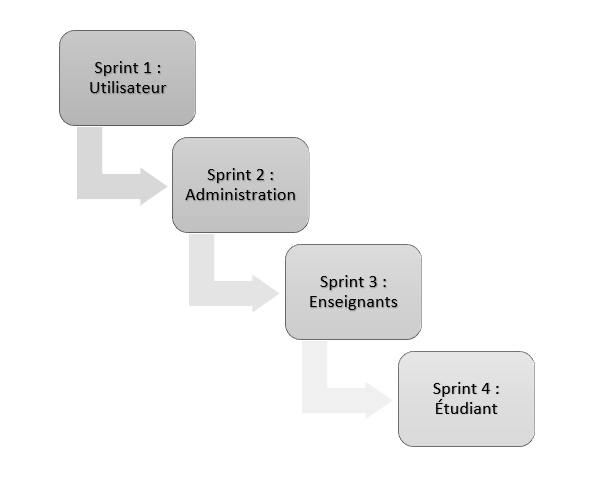
\includegraphics[width=10cm,height=8cm]{Sanstfjitre.png}
	\caption{Section de chapitre 3.}
	\label{fig:Section de chapitre 3}
\end{figure}
\FloatBarrier
\clearpage

\section{Sprint 1 : Utilisateur }
\label{sec:conception}

\begin{fquote}
Ce premier sprint s’étale sur 18 jours et se décompose en trois items  \end{fquote}
\smallskip
\begin{itemize}[label=$\diamond$]
	\item Authentification
	\item Gérer le profil
	\item Modification de rôle
\end{itemize}
\medskip
\medskip
\medskip
\medskip
\medskip
\medskip
\medskip
\medskip
\medskip
\medskip
\begin{figure}[ht]
	\centering
	\includegraphics[width=13cm,height=10cm]{Décompositionsprint1enItems.png}
	\caption{Décomposition sprint 1 en Items.}
	\label{fig:Décomposition sprint 1 en Items}
\end{figure}
\FloatBarrier
\clearpage

\begin{table}[]
	{\Large \color{cyan} Le backlog du sprint 2 est le suivant :}\\
	
	\begin{tabular}{|l|l|l|l|}
		\hline 
		\rowcolor{-blue!20!red}{Item}           & \textbf{User Story}                                                   & \textbf{Description}                                                                                               & \textbf{Priorité} \\ \hline
		\textbf{s'authentifier}                    & s'authentifier                                                            &  je dois m'identifier 
		pour acceder a mon espace                                                                       & 1    \\ \hline
		
		\multirow{4}{*}{\textbf{gérer profil}} & \begin{tabular}[c]{@{}l@{}}Consulter\\ profil\end{tabular}            & \begin{tabular}[c]{@{}l@{}}En tant qu'utilisateur je peux consulter mon \\ profil\end{tabular}                    & 3                 \\ \cline{2-4} 
		& Modifier profil                                                       & \begin{tabular}[c]{@{}l@{}}En tant qu'utilisateur je peux modifier mon \\ profil\end{tabular}                     &                   \\ \cline{2-4} 
		& \begin{tabular}[c]{@{}l@{}}Modifier\\ image de \\ profil\end{tabular} & \begin{tabular}[c]{@{}l@{}}En tant qu'utilisatuer je peux uploader modifier\\ une image de profil\end{tabular}    &                   \\ \cline{2-4} 
		& Désactiver profil                                                     & \begin{tabular}[c]{@{}l@{}}En tant qu'utilisateur je peux désactiver mon\\ profil\end{tabular}                    &                   \\ \hline
		
		\textbf{s'inscrire}                    & s'inscrire                                                            & En tant qu'utilisateur, je peux m'inscrire                                                                        & 1    \\ \hline
	\end{tabular}
	
	
	\caption{Tables Backlog du sprint 2}
	\label{Tables Backlog du sprint 2}
\end{table}
% \section{end_tableau}

\begin{table}[h]
	{\Large \color{cyan} les user stories de sprint 2:}\\
	
	\begin{center}
		\begin{tabular}{>{\begin{bf} } c <{\end{bf}}ccc}
			
			\rowcolor{-blue!20!red}ID U.S & \begin{bf}User Story \end{bf}  & \\
			
			
			1.1  & En tant qu’utilisateur, je dois m’authentifier pour accéder à mon espace \\& \\
			1.2  & En tant qu’utilisateur, je peux m’inscrire \\& \\
			2.1 & En tant qu’utilisateur je peux uploader une image de profil \\& \\
			2.2  & En tant qu’utilisateur je peux afficher mon profil \\& \\
			2.3  & En tant qu’utilisateur je peux modifier mon profil \\& \\
			2.4 & En tant qu’utilisateur je peux désactiver mon profil \\
			
			
		\end{tabular}
	\end{center}
	\caption{Tables  "les user stories de sprint 2"}
	\label{les user stories de sprint 2}
\end{table}
		

\clearpage

\subsection{item 1 : Authentification}
\subsubsection{Diagramme de cas d’utilisation }


\begin{figure}[ht]
	\centering
	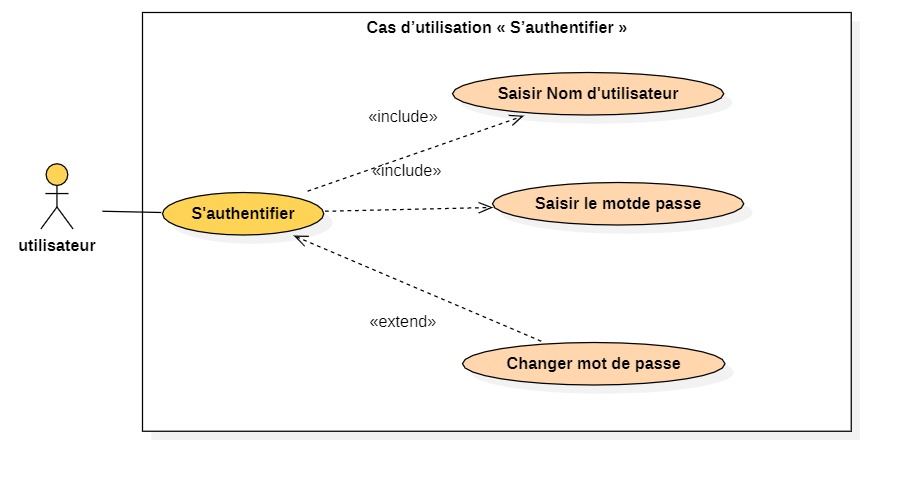
\includegraphics[width=13cm,height=10cm]{DiagrammedeCasdutilisationSauthentifier.png}
	\caption{Diagramme de Cas d' utilisation S' authentifier .}
\label{fig:Diagramme de Cas d utilisation S' authentifier }
\end{figure}
\FloatBarrier

\subsubsubsection{Description détaillée des cas d’utilisations}




\begin{itemize}
	
	\item[$\bullet$] \textbf{Cas d’utilisation S’authentifier :} permet aux utilisateurs de se connecter au système avec leurs logins et mots de passe afin de sécuriser la platforme.
	\medskip
	\begin{itemize}
		\item \textit{\textbf{Objectif :}}  Cette fonctionnalité permet aux différents acteurs de se connecter. 
		
		\item \textit{\textbf{Acteur :}} Tous les acteurs
		
		\item \textit{\textbf{Pré-condition  :}} L’utilisateur existe dans la base de données.
		\item \textit{\textbf{Post-conditions   :}} Utilisateur authentifié.
		\item \textit{\textbf{Scénario nominal :}}
		\begin{enumerate}
			\item L’acteur saisit son login et son mot de passe. 
			\item Le système vérifie les informations saisies. 
			\item Le système trouve que les informations saisies sont valides.  
			\item Le système vérifie le rôle de l’acteur.  
			\item Le système connecte l’acteur à son espace.
		\end{enumerate}
		\item \textit{\textbf{Scénario d'erreur :}} 
		\begin{enumerate}
			\item L’acteur saisit son login et son mot de passe. 
			\item Le système vérifie les informations saisies.   
			\item Le système trouve que les informations saisies sont invalides.  
			\item Le système demande à l’acteur de vérifier les informations saisies.
		\end{enumerate}
	\end{itemize}	
	\bigskip
\end{itemize}
\bigskip
\subsubsection{Diagrammes de séquence système }
\begin{figure}[ht]
	\centering
	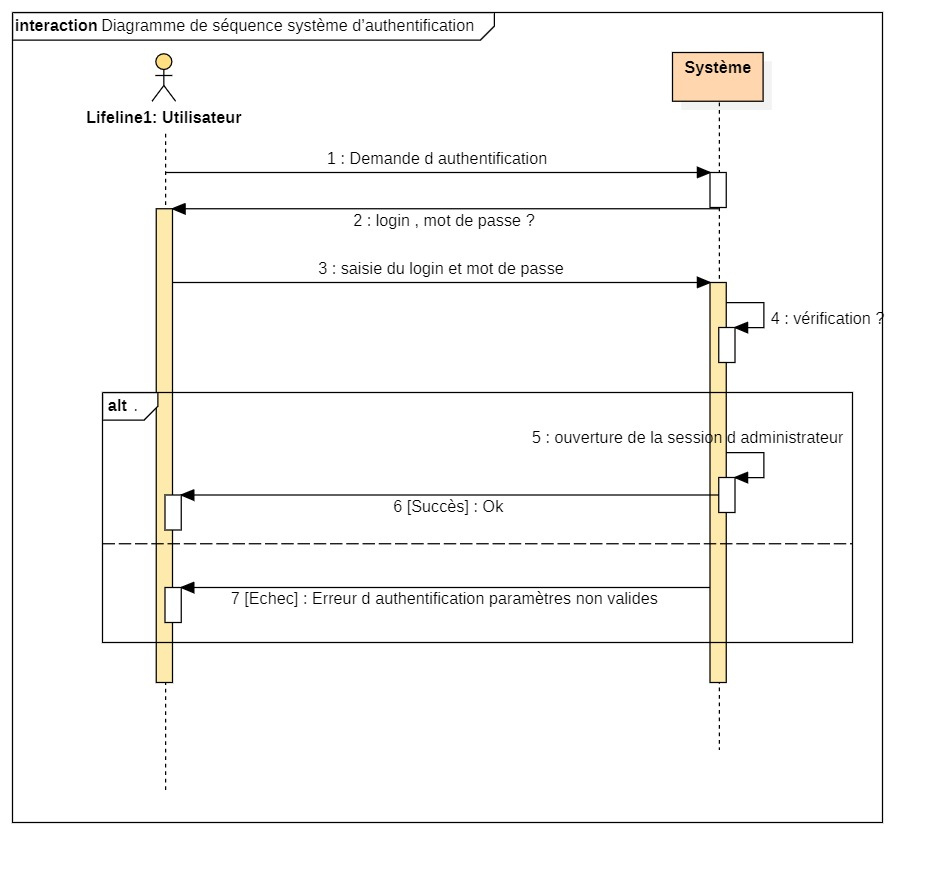
\includegraphics[width=13cm,height=10cm]{Diagrséquencesystèmeauthentification.jpg}
	\caption{Diagramme de séquence système d' authentification .}
	\label{fig:Diagramme de séquence système d' authentification }
\end{figure}
\FloatBarrier

\subsubsection{ Interface : Gérer le profil  }


\begin{figure}[ht]
	\centering
	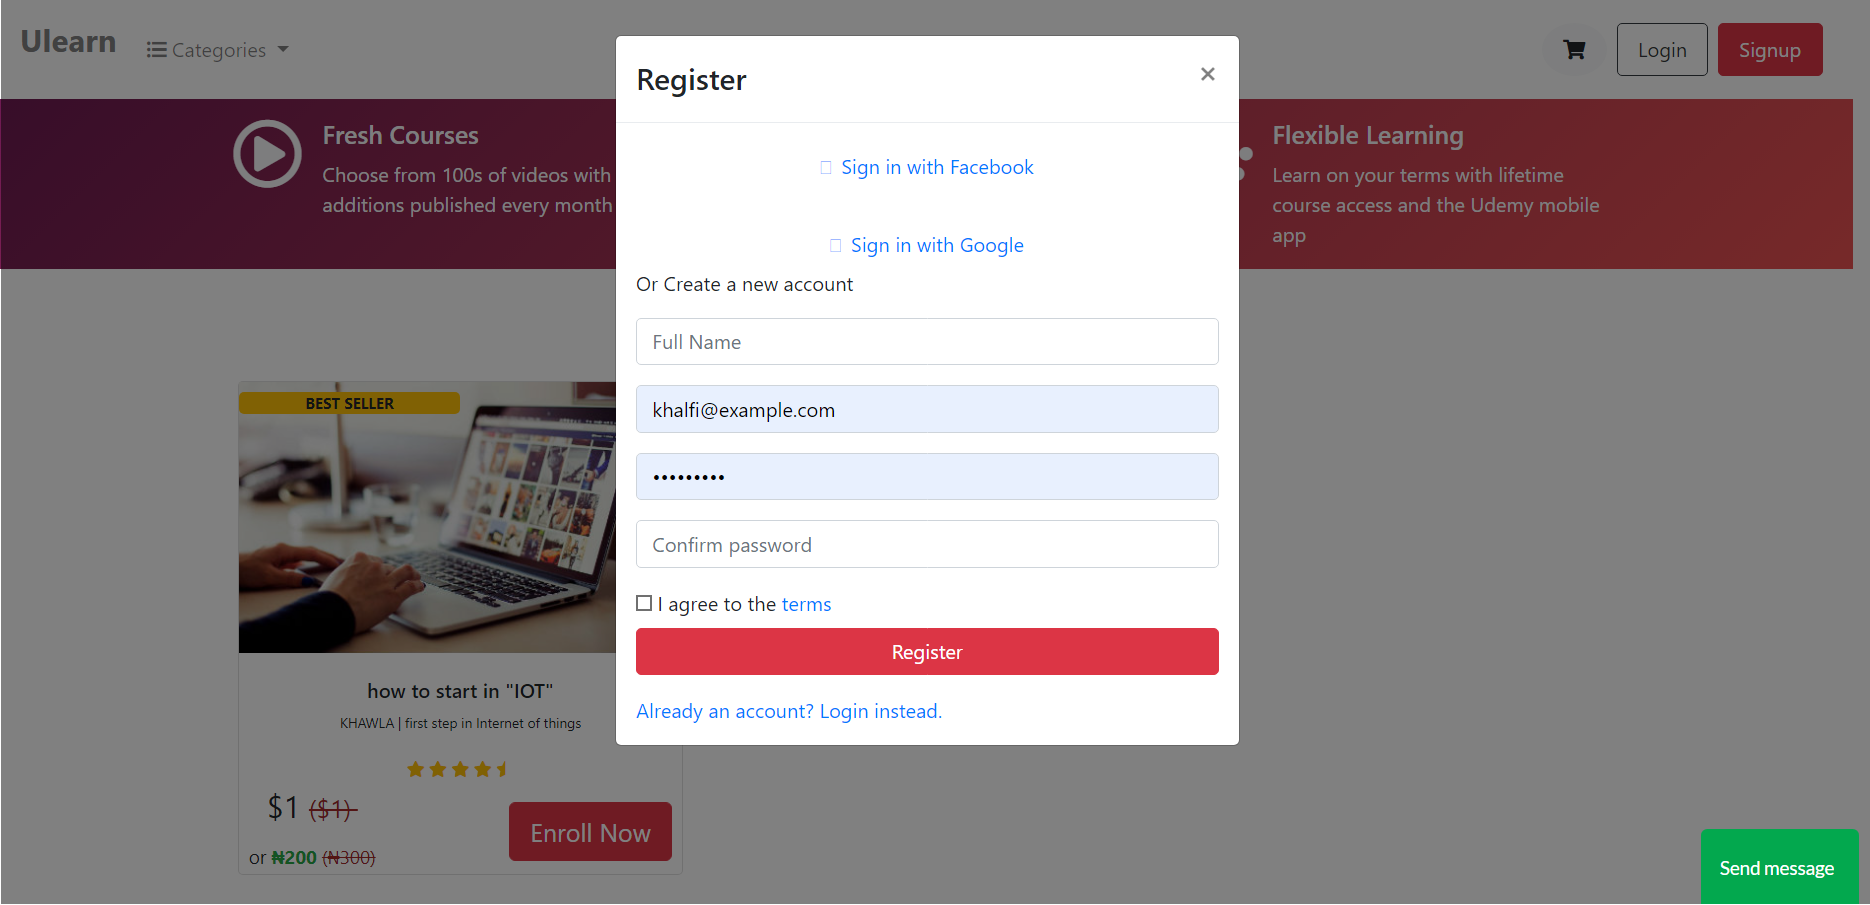
\includegraphics[width=17cm,height=8cm]{20.png}
	\caption{Interface : Gérer le profil .}
	\label{fig:Interface : Gérer le profil }
\end{figure}
\FloatBarrier
\begin{figure}[ht]
	\centering
	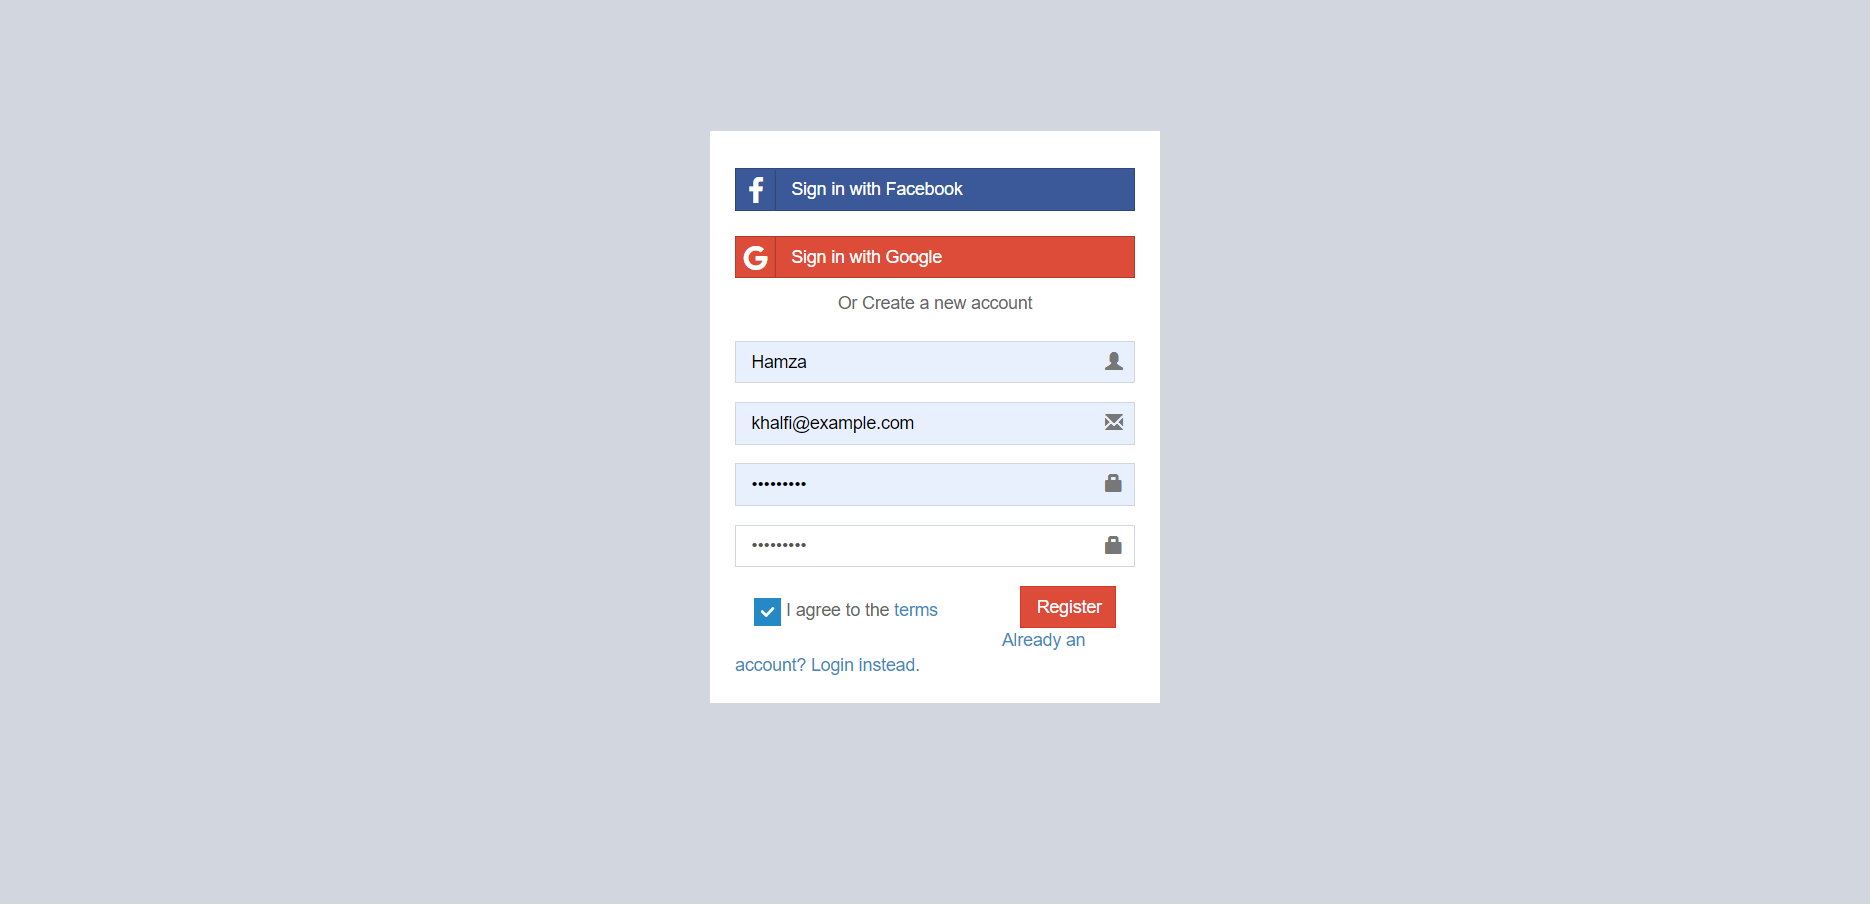
\includegraphics[width=17cm,height=9cm]{21.png}
	\caption{Interface : Gérer le profil .}
	\label{fig:Interface : Gérer le profil }
\end{figure}
\FloatBarrier
\clearpage
\subsection{item 2 : Gérer le profil}
\subsubsection{Diagramme de cas d’utilisation }


\begin{figure}[ht]
	\centering
	\includegraphics[width=13cm,height=10cm]{CasutilisationGérprofil.jpg}
	\caption{Diagramme de Cas d' utilisation Gérer le profil .}
	\label{fig:Gérer le profil }
\end{figure}
\FloatBarrier


\begin{itemize}
	
	\item[$\bullet$] \textbf{Cas d’utilisation Gérer le profil :} permet à l’acteur de mettre à jour ses informations.
	\medskip
	\begin{itemize}
		\item \textit{\textbf{Objectif :}}  Cette fonctionnalité permet aux différents acteurs de mettre à jour ses informations. 
		
		\item \textit{\textbf{Acteur :}} Tous les acteurs
		
		\item \textit{\textbf{Pré-condition  :}}  L‘acteur doit être un membre identifié.
		\item \textit{\textbf{Post-conditions   :}} le cas démarre après le point 02 de l’enchainement nominal.
		\item \textit{\textbf{Scénario nominal :}}
		\begin{enumerate}
			\item le système affiche le profil actuel de l’acteur. 
			\item l’acteur met à jour ses informations. 
			\item  le système vérifie la validité des informations saisies.  
			\item  le système enregistre ces informations dans la base de données .  
			\item le système notifie l’acteur du bon déroulement de mise à jour de son profil
		\end{enumerate}
		\item \textit{\textbf{Scénario alternative :}} \\
			les informations sont manquantes ou incorrectes: ce scénario commence au point 03 du
		scénario nominal.
		\begin{enumerate}
		
			\item Le système informe l’acteur que les données saisies sont erronées, garde les informations
			saisies avant et le scénario reprend au point 02 du scénario nominal. 
		\end{enumerate}
	\end{itemize}
\end{itemize}	
	\bigskip


\subsubsection{ Interface : Gérer le profil  }


\begin{figure}[ht]
	\centering
	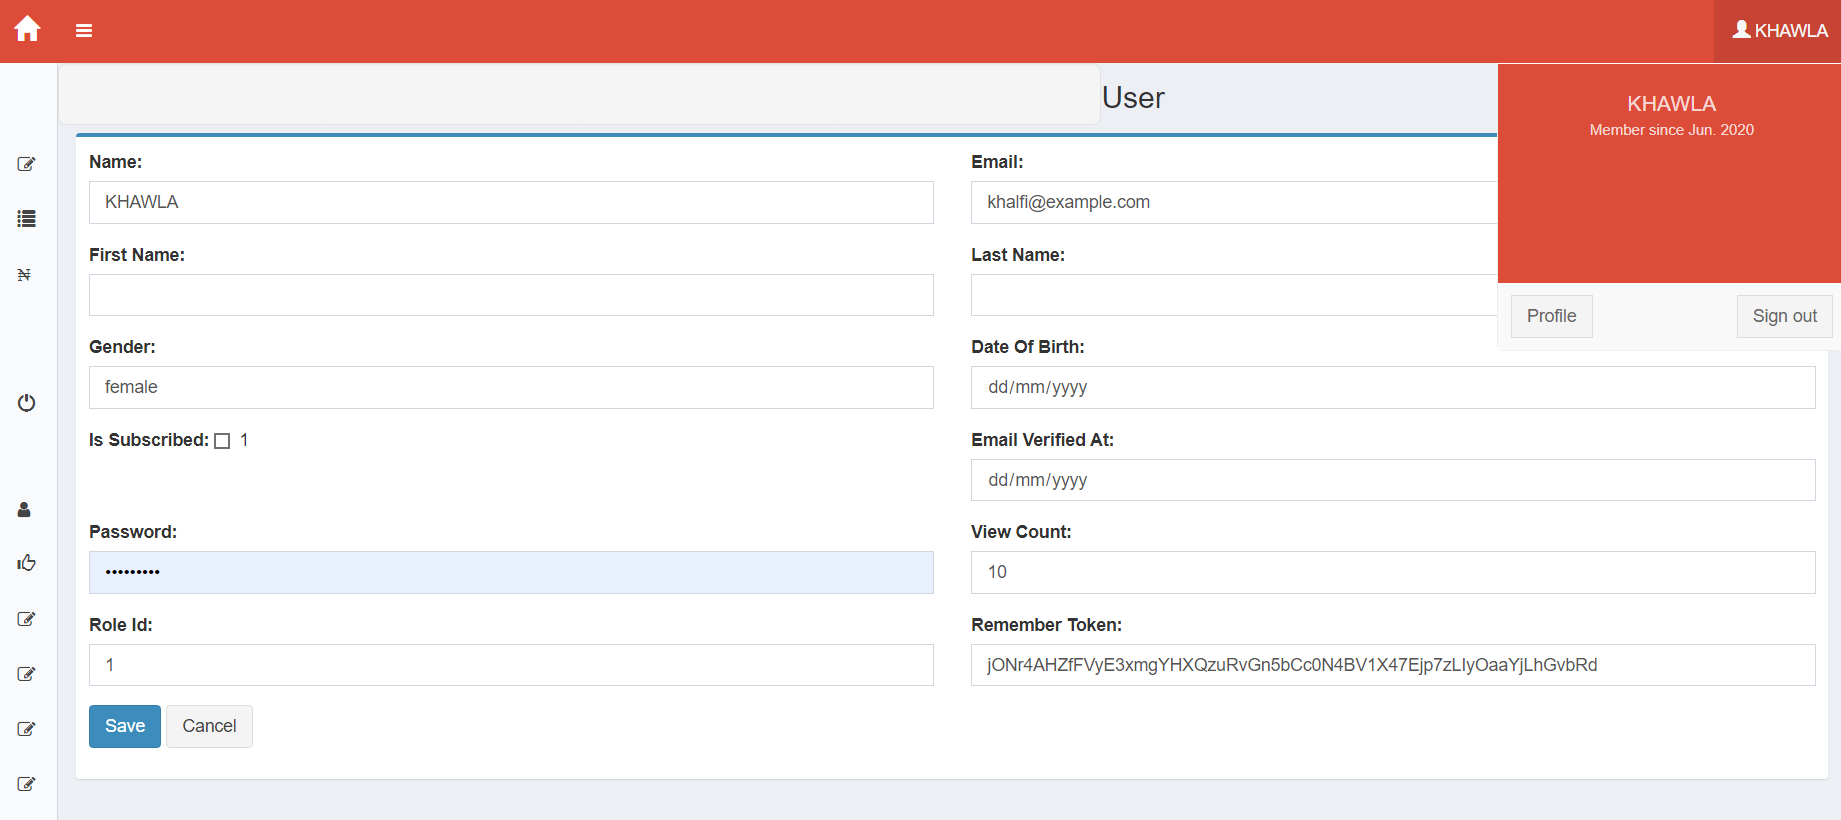
\includegraphics[width=17cm,height=13cm]{OperaSnapshot.png}
	\caption{Interface : Gérer le profil .}
	\label{fig:Interface : Gérer le profil }
\end{figure}
\FloatBarrier










\clearpage
\subsection{item 3 : Modification de rôle}
\subsubsection{Diagrammes de séquence système }


\begin{figure}[ht]
	\centering
	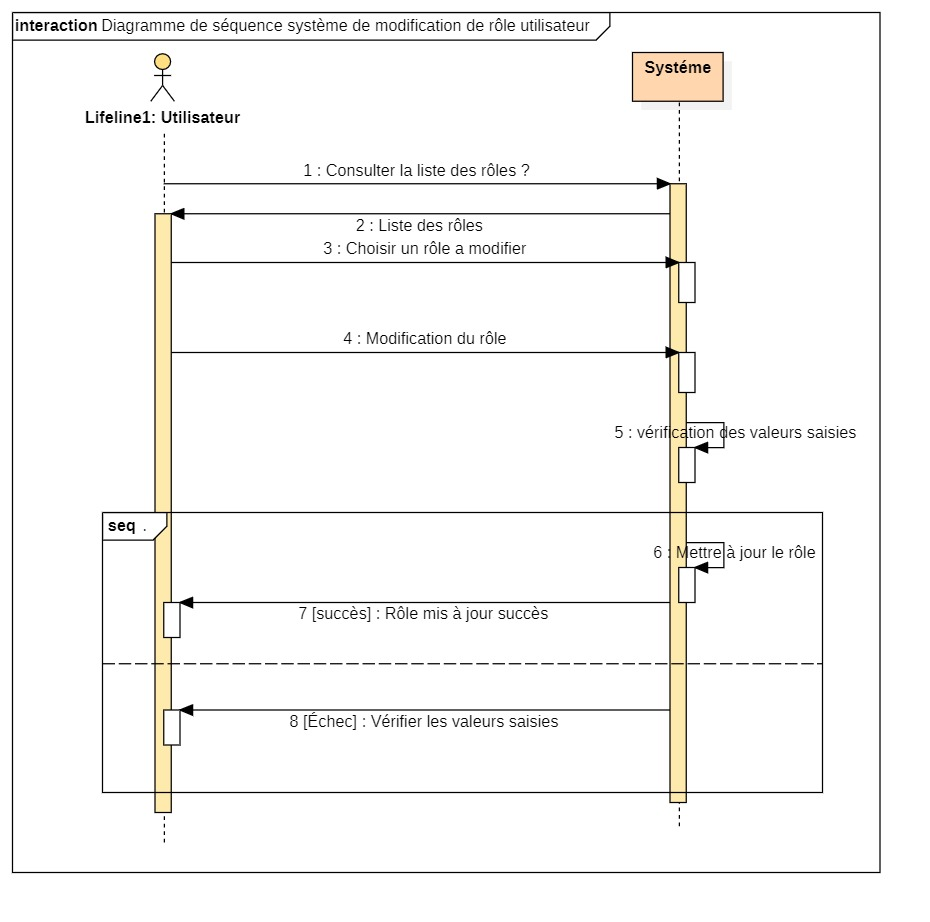
\includegraphics[width=13cm,height=10cm]{Diagséquencesystèmedemodificationderôleutilisateur.jpg}
	\caption{Diagramme de séquence système de modification de rôle utilisateur .}
	\label{fig:Diagramme de séquence système de modification de rôle utilisateur }
\end{figure}
\FloatBarrier
\clearpage
\subsubsection{ Interface : Gérer le profil  }
\begin{figure}[ht]
	\centering
	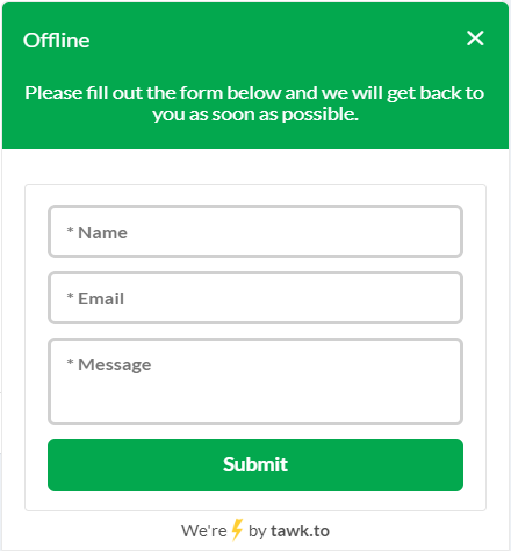
\includegraphics[width=13cm,height=10cm]{3.png}
	\caption{Diagramme de séquence système de modification de rôle utilisateur .}
	\label{fig:Diagramme de séquence système de modification de rôle utilisateur }
\end{figure}
\FloatBarrier
\begin{figure}[ht]
	\centering
	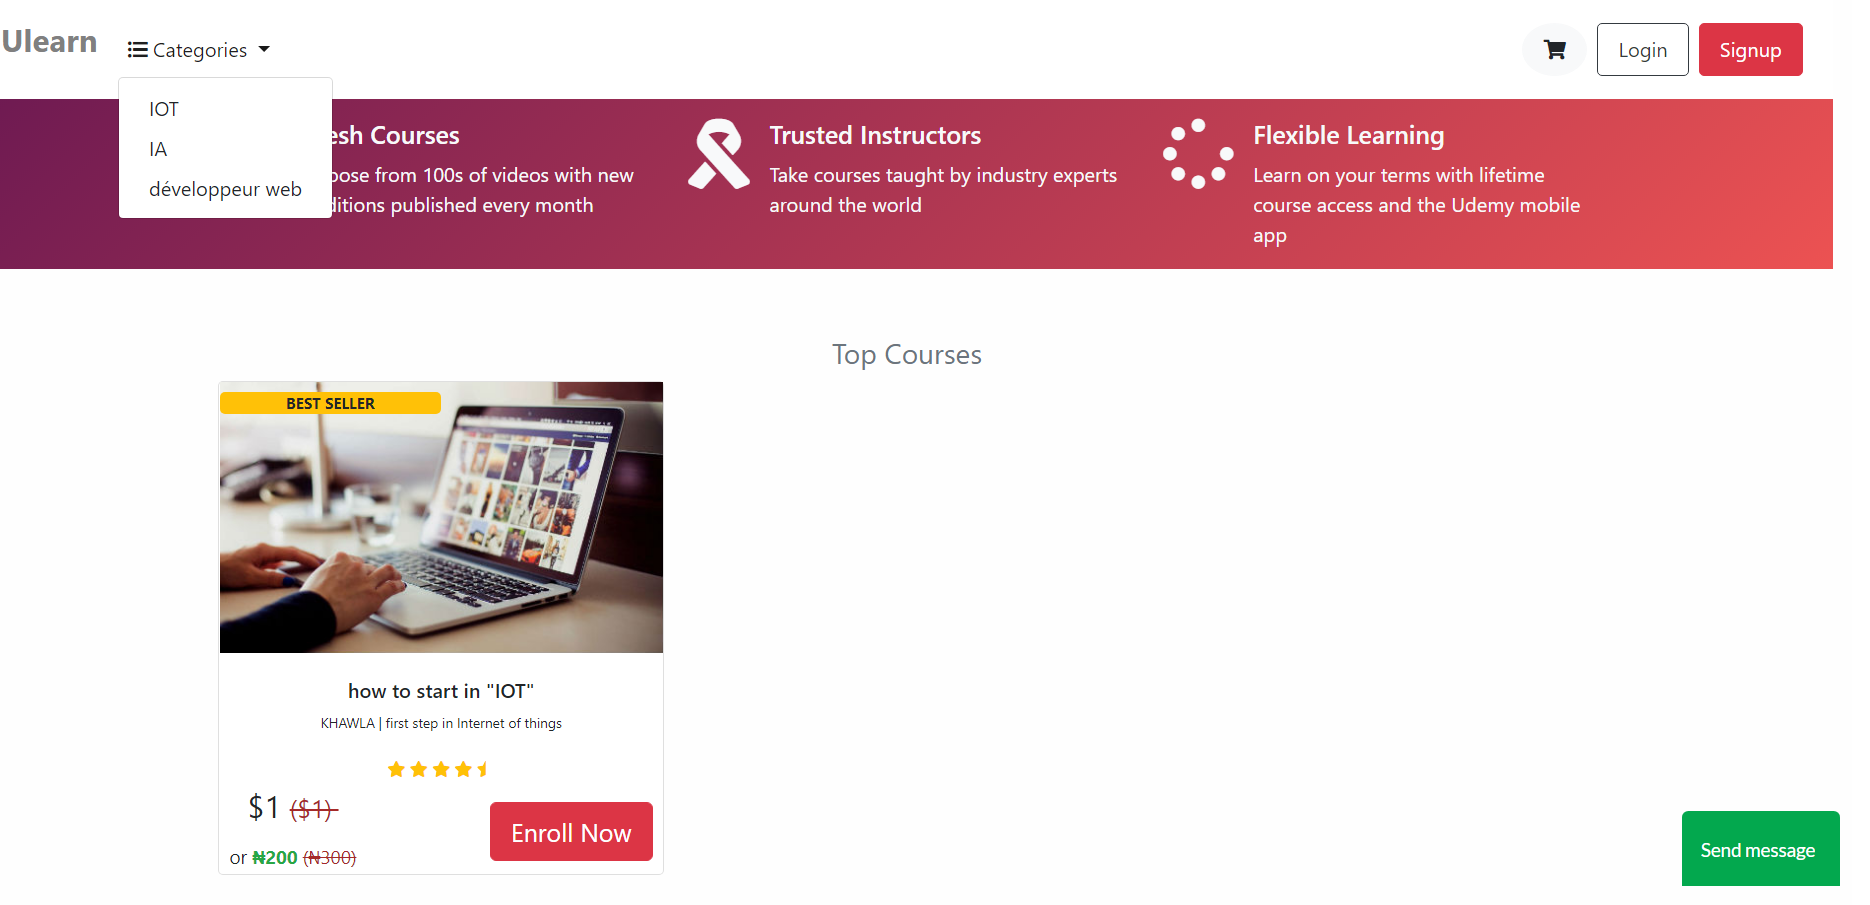
\includegraphics[width=13cm,height=10cm]{18.png}
	\caption{Diagramme de séquence système de modification de rôle utilisateur .}
	\label{fig:Diagramme de séquence système de modification de rôle utilisateur }
\end{figure}
\FloatBarrier
\clearpage



\section{Sprint 2 : Administration }



\begin{fquote}
Ce premier sprint s’étale sur 26 jours et se décompose en deux items \end{fquote}
\smallskip
\begin{itemize}[label=$\diamond$]
	\item Gérer les utilisateurs
    \item  Inscription et réinscription d'un étudiant
	
\end{itemize}
\medskip
\medskip
\medskip
\medskip
\medskip
\medskip
\medskip
\medskip
\medskip
\medskip
\medskip
\begin{figure}[ht]
	\centering
	\includegraphics[width=13cm,height=10cm]{Décompositionsprint2enItems.png}
	\caption{Décomposition sprint 2 en Items.}
	\label{fig:Décomposition sprint 2 en Items}
\end{figure}
\FloatBarrier
\clearpage




\begin{table}[]
	{\Large \color{cyan} Le backlog du sprint 2 est le suivant :}\\
	
	\begin{tabular}{|l|l|l|l|}
		\hline 
		\rowcolor{-blue!20!red}{Item}           & \textbf{User Story}                                                   & \textbf{Description}                                                                                               & \textbf{Priorité} \\ \hline
		\textbf{s'authentifier}                    & s'authentifier                                                            &  je dois m'identifier 
			 pour acceder a mon espace                                                                       & 1    \\ \hline
	
		\multirow{4}{*}{\textbf{gérer profil}} & \begin{tabular}[c]{@{}l@{}}Consulter\\ profil\end{tabular}            & \begin{tabular}[c]{@{}l@{}}En tant qu'utilisateur je peux consulter mon \\ profil\end{tabular}                    & 3                 \\ \cline{2-4} 
		& Modifier profil                                                       & \begin{tabular}[c]{@{}l@{}}En tant qu'utilisateur je peux modifier mon \\ profil\end{tabular}                     &                   \\ \cline{2-4} 
		& \begin{tabular}[c]{@{}l@{}}Modifier\\ image de \\ profil\end{tabular} & \begin{tabular}[c]{@{}l@{}}En tant qu'utilisatuer je peux uploader modifier\\ une image de profil\end{tabular}    &                   \\ \cline{2-4} 
		& Désactiver profil                                                     & \begin{tabular}[c]{@{}l@{}}En tant qu'utilisateur je peux désactiver mon\\ profil\end{tabular}                    &                   \\ \hline
		
		\textbf{s'inscrire}                    & s'inscrire                                                            & En tant qu'utilisateur, je peux m'inscrire                                                                        & 1    \\ \hline
	\end{tabular}
	
	
	\caption{Tables Backlog du sprint 2}
	\label{Tables Backlog du sprint 2}
\end{table}
% \section{end_tableau}

\begin{table}[h]
{\Large \color{cyan} les user stories de sprint 2:}\\
	
	\begin{center}
		\begin{tabular}{>{\begin{bf} } c <{\end{bf}}ccc}
			
			\rowcolor{-blue!20!red}ID U.S & \begin{bf}User Story \end{bf}  & \\
			
			
			1.1  & En tant qu’utilisateur, je dois m’authentifier pour accéder à mon espace \\& \\
		1.2  & En tant qu’utilisateur, je peux m’inscrire \\& \\
			2.1 & En tant qu’utilisateur je peux uploader une image de profil \\& \\
			2.2  & En tant qu’utilisateur je peux afficher mon profil \\& \\
			2.3  & En tant qu’utilisateur je peux modifier mon profil \\& \\
			2.4 & En tant qu’utilisateur je peux désactiver mon profil \\
			
			
		\end{tabular}
	\end{center}
	\caption{Tables  "les user stories de sprint 2"}
	\label{les user stories de sprint 2}
\end{table}


\clearpage

\clearpage
 
\subsection{item 1 : Gérer les utilisateurs}
\subsubsection{Diagramme de cas d’utilisation  détaillé «administrer du site de téléformation» }

\begin{figure}[ht]
	\centering
	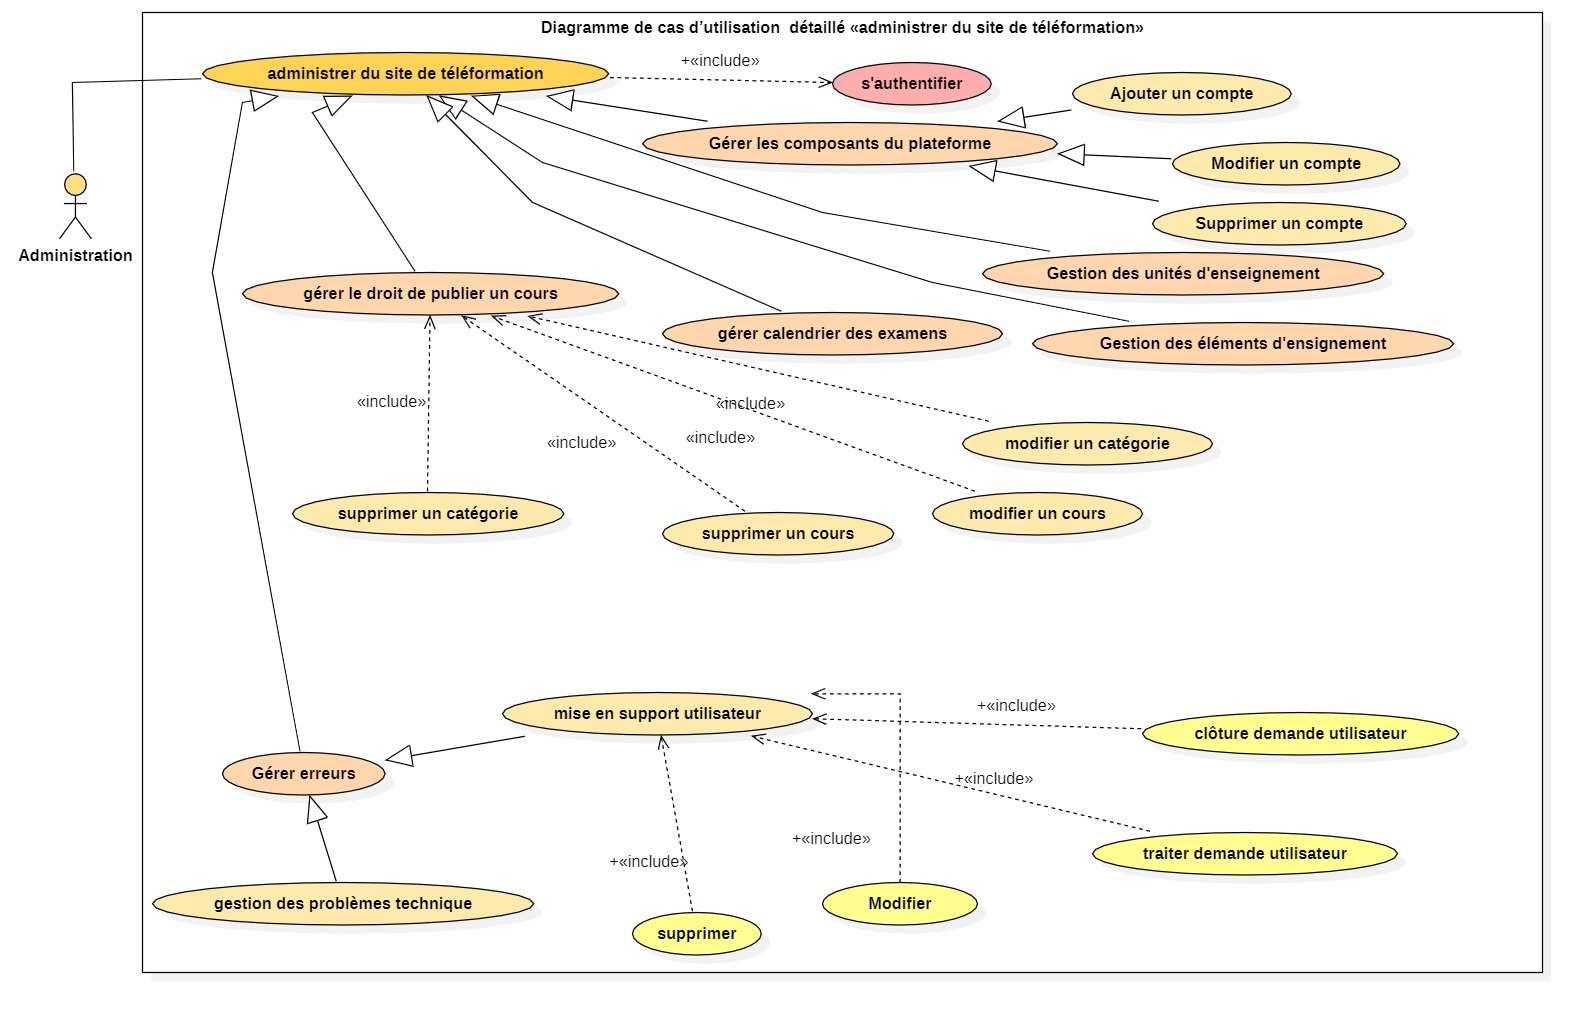
\includegraphics[width=13cm,height=10cm]{Diagrammedecasdutilisationdétailléadministr.jpg}
	\caption{Diagramme de cas d' utilisation  détaillé «administrer» .}
	\label{fig:Diagramme de cas d' utilisation  détaillé administrer  }
\end{figure}
\FloatBarrier

\subsubsubsection{Description détaillée des cas d’utilisations}
L'administrateur a comme rôle principale de gérer toutes les taches de la plateforme; gestion des enseignants, étudiants ,matières....ainsi que les affectations des
enseignants.\\
L'administrateur peut ajouter, supprimer ou modifier les différentes informations des étudiants d'une manière permanente.\\
L'administrateur peux dérer des droits et des erreures .

\begin{itemize}
      \item[$\bullet$] \textbf{Cas d’utilisation Gérer le profil :} permet à l’acteur de mettre à jour la plateforme. 
	\medskip
	\begin{itemize}
		\item \textit{\textbf{Objectif :}}  permet à l’administrateur de modifier la composition interne de la plateforme. 
		
		\item \textit{\textbf{Acteur :}} Administrateur
		
		\item \textit{\textbf{Pré-condition  :}}  L‘acteur doit être connecté.
		\item \textit{\textbf{Post-conditions   :}}
		\item \textit{\textbf{Scénario nominal :}}
		\begin{enumerate}
			\item le système affiche l’état actuel de la plateforme. 
			\item l’acteur met à jour la plateforme. 
			\item   le système vérifie la validité des mis à jour.  
			\item  le système enregistre les mis à jours dans la base de données.  
			\item le système notifie l’acteur du bon déroulement de mise à jour de la plateforme.
		\end{enumerate}
		\item \textit{\textbf{Scénario alternative :}} \\
les informations sont manquantes ou incorrectes: ce scénario commence au point 03 du
scénario nominal
		\begin{enumerate}
			\item  Le système informe l’acteur que les mis à jour sont erronées, garde l’état de la plateforme 
		\end{enumerate}
	\end{itemize}
\end{itemize}	
\bigskip





\subsubsubsection{Description détaillée des cas d’utilisations}
\begin{itemize}
	\item[$\bullet$] \textbf{Cas d’utilisation Gérer les utilisateurs :} 
	\medskip
	\begin{itemize}
		\item \textit{\textbf{Objectif :}} permet à l’acteur d’ajouter et de supprimer un utilisateur. 
		
		\item \textit{\textbf{Acteur :}} Administrateur
		
		\item \textit{\textbf{Pré-condition  :}} L‘acteur doit être connecté.
		\item \textit{\textbf{Post-conditions   :}}
		\item \textit{\textbf{Scénario nominal :}}
		\begin{enumerate}
			\item Le système affiche un formulaire d’inscription à l’acteur. 
			\item L’acteur saisit les informations du nouvel utilisateur et lui affecter un rôle. 
			\item    Le système vérifie la validité des informations saisies. 
			\item  Le système enregistre ces informations dans la base de données.  
			\item Le système notifie l’acteur du bon déroulement de l’inscription..
		\end{enumerate}
		\item \textit{\textbf{Scénario alternative :}} \\
les informations sont manquantes ou incorrectes: ce scénario commence au point 03 du
scénario nominal.
		\begin{enumerate}
			\item  Le système informe l’acteur que les données saisies sont erronées et le scénario reprend au point 02 du scénario nominal.
		\end{enumerate}
	\end{itemize}
\end{itemize}	
\bigskip
\subsubsection{Diagrammes de séquence du cas d' utilisation "Modifier un utilisateur" }
\begin{figure}[ht]
	\centering
	\includegraphics[width=13cm,height=10cm]{DiagrammesdeséquenceducasdutilisationModifierunutilisa.jpg}
	\caption{Diagrammes de séquence du cas d' utilisation "Modifier un utilisateur"  .}
	\label{fig:Diagrammes de séquence du cas d' utilisation Modifier un utilisateur }
\end{figure}
\FloatBarrier
\subsubsubsection{Description détaillée des cas d’utilisations}
\begin{itemize}
	\item[$\bullet$] \textbf{Cas d’utilisation "Modifier un utilisateur" :} 
	\medskip
	\begin{itemize}
		\item \textit{\textbf{Objectif :}} Modifier un utilisateur 	
		\item \textit{\textbf{Acteur :}} Administrateur	
		\item \textit{\textbf{Pré-condition  :}} Authentification préalable.\\
		Utilisateur existant.\\
		Formulaire d’ajout disponible.
\\
		\item \textit{\textbf{Post-conditions   :}}L’utilisateur a bien été modifié .
		\item \textit{\textbf{Scénario nominal :}}
		\begin{enumerate}
			\item L’utilisateur demande le formulaire de modification d’un utilisateur.
			\item Le système affiche le formulaire avec l’ensemble des anciennes informations de l’utilisateur.
			\item L’administrateur modifie les champs nécessaires. 
			\item Le système vérifie les données saisies. 
			\item L’administrateur valide la modification . 
			\item Le système vérifie l’existence de l’utilisateur .  
			\item Le système modifie l’utilisateur.
		\end{enumerate}
		\item \textit{\textbf{Scénario alternative :}}
		\begin{enumerate}
			\item L’utilisateur saisit des informations manquantes ou erronées.
			\item  Le système renvoie un message d’erreur adéquat.
			\item Reprise de l’étape 3 du scénario Nominal.
		\end{enumerate}
	\end{itemize}
\end{itemize}	
\bigskip
\subsubsection{Diagramme de séquence du cas d' utilisation "Supprimer un utilisateur" }
\begin{figure}[ht]
	\centering
	\includegraphics[width=13cm,height=10cm]{DiagrammedeséquenceducasdutilisationSupprimerunutilisateur.jpg}
	\caption{ Diagramme de séquence du cas d' utilisation "Supprimer un utilisateur"  .}
	\label{fig: Diagramme de séquence du cas d' utilisation Supprimer un utilisateur  }
\end{figure}
\FloatBarrier
\subsubsubsection{Description détaillée des cas d’utilisations}
\begin{itemize}
	\item[$\bullet$] \textbf{Cas d’utilisation "Supprimer un utilisateur" :} 
	\medskip
	\begin{itemize}
		\item \textit{\textbf{Objectif :}} Supprimer un utilisateur	
		\item \textit{\textbf{Acteur :}} Administrateur	
		\item \textit{\textbf{Pré-condition  :}} Authentification préalable.\\
		Utilisateur existant.
		\item \textit{\textbf{Post-conditions   :}}L’utilisateur a bien été supprimé.
		\item \textit{\textbf{Scénario nominal :}}
		\begin{enumerate}
			\item L’administrateur choisit l’utilisateur à supprimer. 
			\item Le système affiche un message de confirmation. 
			\item  L’administrateur valide son choix . 
			\item  Le système supprime l’utilisateur.  
			\item Le système affiche un message de succès.
		\end{enumerate}
		\item \textit{\textbf{Scénario alternative :}}
		\begin{enumerate}
			\item Le L’administrateur annule son choix.
			\item Le système annule la suppression.
		\end{enumerate}
	\end{itemize}
\end{itemize}	
\bigskip
\subsubsection{Diagrammes de séquence du cas d' utilisation "Ajouter un utilisateur" }
\begin{figure}[ht]
	\centering
	\includegraphics[width=13cm,height=10cm]{DiagrammesdeséquenceducasdutilisationAjouterunutilisateur.jpg}
	\caption{Diagrammes de séquence du cas d' utilisation "Ajouter un utilisateur"  .}
	\label{fig:Diagrammes de séquence du cas d' utilisation Ajouter un utilisateur  }
\end{figure}
\FloatBarrier
\subsubsubsection{Description détaillée des cas d’utilisations}
\begin{itemize}
	\item[$\bullet$] \textbf{Cas d’utilisation "Ajouter un utilisateur" :} 
	\medskip
	\begin{itemize}
		\item \textit{\textbf{Objectif :}} Ajouter un utilisateur pour qu’il avoir l’accés au fonctionnalités de l’espace	
		\item \textit{\textbf{Acteur :}} Administrateur	
		\item \textit{\textbf{Pré-condition  :}} Authentification préalable.\\
		Un formulaire d’ajout des utilisateurs est disponible.
		\item \textit{\textbf{Post-conditions   :}}Un nouvel utilisateur ajouté.
		\item \textit{\textbf{Scénario nominal :}}
		\begin{enumerate}
			\item L’administrateur demande un formulaire d’ajout d’un nouveau utilisateur.
			\item Le système affiche le formulaire d’ajout.
			\item L’administrateur doit remplir le formulaire avec l’ensemble des informations
			nécessaires à l’ajout du nouvel utilisateur. 
			\item Le système vérifie les données saisies. 
			\item  L’administrateur valide . 
			\item  Le système vérifie l’existence du nouveau compte .  
			\item Le système enregistre les informations saisies du l’utilisateur.
		\end{enumerate}
		\item \textit{\textbf{Scénario alternative :}}
		\begin{enumerate}
			\item L’utilisateur saisit les informations manquantes ou erronées.
			\item Le système affiche un ou des message d’erreurs selon les champs invalides.
			\item Reprise de l’étape 3 du scénario nominal.
			\item L’utilisateur existe déjà.
			\item Le système informe l’administrateur que l’utilisateur existe déjà dans le système.
			\item Reprise de l’étape 3 du scénario nominal.
		\end{enumerate}
	\end{itemize}
\end{itemize}	
\bigskip
\subsubsection{Diagramme de séquence « d' ajout d'un professeur » }
\begin{figure}[ht]
	\centering
	\includegraphics[width=13cm,height=10cm]{Diagrammedeséquencedajoutdunprofesseur.jpg}
	\caption{Diagramme de séquence « d' ajout d'un professeur »  .}
	\label{fig:Diagramme de séquence  d' ajout d'un professeur   }
\end{figure}
\FloatBarrier
\subsubsubsection{Description détaillée des cas d’utilisations}



\begin{itemize}
	\item[$\bullet$] \textbf{Diagramme de séquence « d' ajout d'un professeur » :} 
	\medskip
	\begin{itemize}
		\item \textit{\textbf{Objectif :}} Permettre à l’administration d’ajouter toutes les informations
		concernant le professeur, y compris les informations personnelles, et la possibilité
		d’ajouter les diplômes obtenus par le professeur .	
		\item \textit{\textbf{Acteur :}} Administrateur	
		\item \textit{\textbf{Pré-condition  :}} Authentification .\\
		L’ajout d’un professeur doit répond aux conditions de recrutement établie par la direction régionale.
		\item \textit{\textbf{Scénario :}}
		\begin{enumerate}
			\item Saisie des informations concernant le professeur.
		\item Contrôle des données en temps réel, en cas de duplication.
		\item Validation de la saisie.
		\item Traitement des informations envoyées.
		\item En cas d’une anomalie, l’ajout est rejeté en précisant l’erreur effectuée.
		\item Si non, l’ajout est effectué avec succès avec redirection d’utilisateur vers la liste des
			professeurs.
		\end{enumerate}
	\end{itemize}
\end{itemize}	
\bigskip








\subsubsection{Diagramme d’activités « Gérer les utilisateurs » }
\begin{figure}[ht]
	\centering
	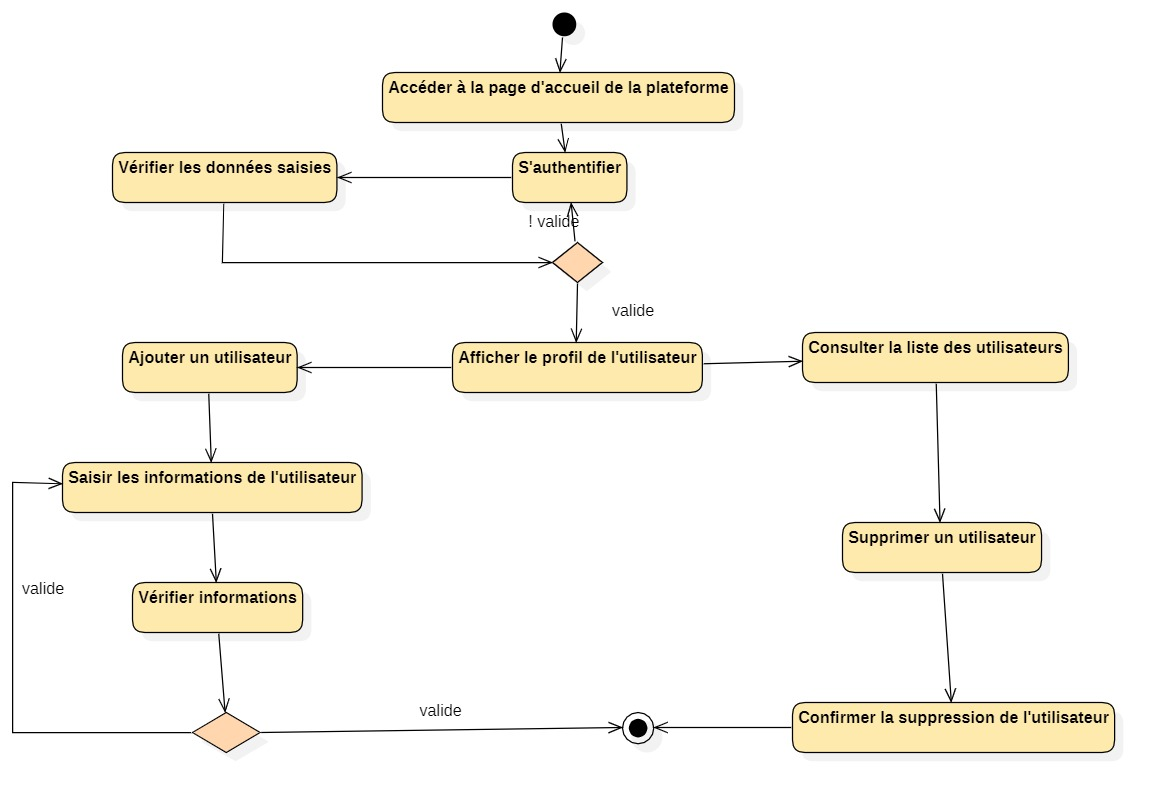
\includegraphics[width=13cm,height=10cm]{DiagrammeactivitésGérerlesutilisateurs.jpg}
	\caption{Diagramme d' activités  « Gérer les utilisateurs »  .}
	\label{fig:Diagramme d' activités  Gérer les utilisateurs  }
\end{figure}
\FloatBarrier

\subsubsubsection{Description détaillée des cas d’utilisations}
La figure ci-dessus illustre le déroulement séquentiel de la gestion des utilisateurs accomplis par
un administrateur .\\
Après avoir s’authentifié, ces derniers peuvent ajouter ou supprimer un utilisateur.\\
Pour l’ajout d’un utilisateur, le système doit vérifier la validation des informations saisies.\\
 Au cas où une information n’est pas valide, le système réaffiche l’interface d’ajout d’un utilisateur.
\clearpage
\subsection{item 2 : Inscription et réinscription d'un étudiant}
\subsubsection{Diagramme de séquence « d' inscription d' un étudiant » }
\begin{figure}[ht]
	\centering
	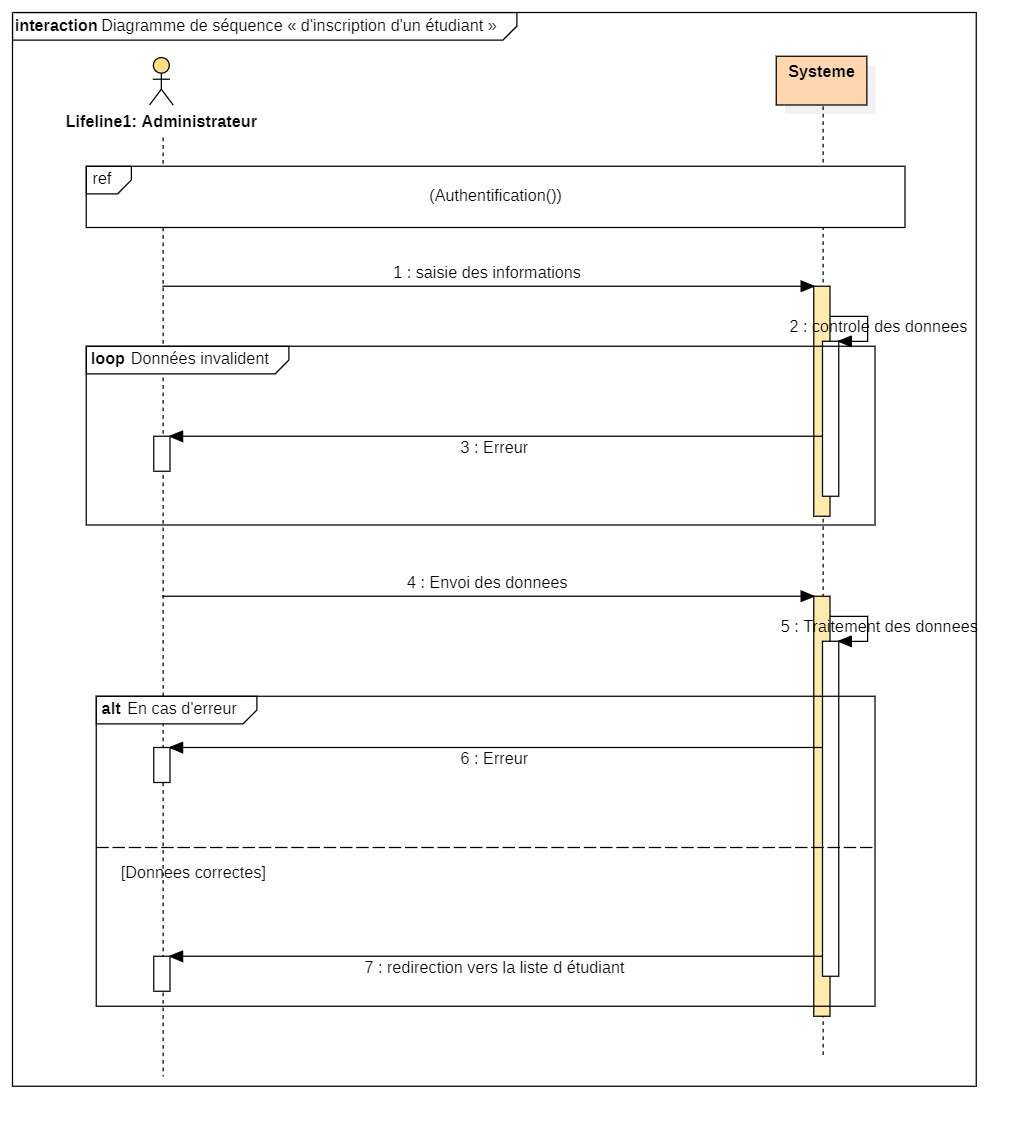
\includegraphics[width=13cm,height=10cm]{Diagrammeséquencenscriptiétudiant.jpg}
	\caption{Diagramme de séquence « d' inscription d' un étudiant » .}
	\label{fig:Diagramme de séquence  d' inscription d' un étudiant   }
\end{figure}
\FloatBarrier

\subsubsubsection{Description : Diagramme de séquence « d' inscription d' un étudiant » }

\begin{itemize}
	\item[$\bullet$] \textbf{Diagramme de séquence « d' inscription d' un étudiant » :} 
	\medskip
	\begin{itemize}
		\item \textit{\textbf{Objectif :}} Permettre à l'administration d'ajouter toutes les informations
		concernant un étudiant, y compris l’état civil, et les
		informations complémentaires .	
		\item \textit{\textbf{Acteur :}} Administrateur	
		\item \textit{\textbf{Pré-condition  :}} Authentification .\\
		L’inscription d’un étudiant doit répond aux conditions d’inscription établie par
		la direction régionale
		\item \textit{\textbf{Scénario :}}
		\begin{enumerate}
		\item Saisie les informations de l’élève.
		\item Contrôle des données en temps réel (matricule – cne – cin) en cas de duplication.
		\item Validation de la saisie.
		\item Traitement des informations envoyé.
		\item En cas d’une anomalie, l’inscription est rejetée on précisant l’erreur effectuée.
		\item Si non, l’inscription est effectuée avec succès avec redirection d’utilisateur vers la
			liste d’élèves.
		\end{enumerate}
	\end{itemize}
\end{itemize}	
\bigskip

















\subsubsection{Diagramme d'activités « d'inscription d'un étudiant» }
\begin{figure}[ht]
	\centering
	\includegraphics[width=13cm,height=10cm]{Diagrammeactivitésinscriptioun.jpg}
	\caption{Diagramme d'activités « d'inscription d'un étudiant» .}
	\label{fig:Diagramme d' activités  d' inscription d'un étudiant   }
\end{figure}
\FloatBarrier

\subsubsubsection{ Description du processus de diagramme d’activités «Inscription d’un élève» :}
\begin{itemize}	
\item[$\star$]L’élève demande l’inscription dans un niveau.
\item[$\star$] L’administration vérifie les conditions d’inscriptions pour l’élève.
\item[$\star$] Si l’élève ne répond pas aux conditions de l’établissement, donc la demande est refusée.
\item[$\star$] Si non, l’élève doit fournir les pièces et les informations nécessaires pour
l’inscription.
\item[$\star$] L’administration donne les informations personnelles de l’élève.
\item[$\star$] L’administration introduit les informations complémentaires et celles concernant la santé de l’élève.
\item[$\star$] L’administration affecte le niveau et valide l’inscription.
\item[$\star$] Le système traite les informations envoyées.
\item[$\star$] En cas d’une anomalie, le système refuse l’inscription demandant à l’administration de vérifier l’anomalie.
\item[$\star$] Si non, l’inscription est effectuée avec succès.
\end{itemize}	
\subsubsection{Diagramme de collaboration «réinscription d' un étudiant»}
\begin{figure}[ht]
	\centering
	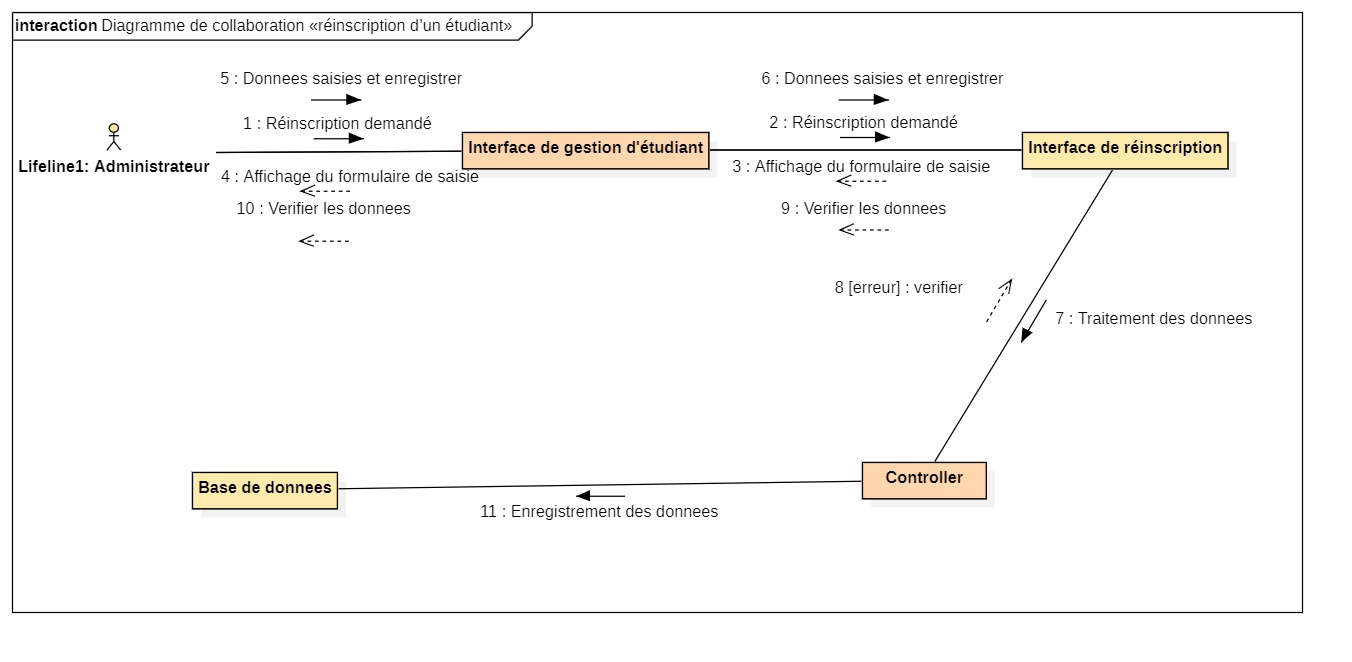
\includegraphics[width=13cm,height=10cm]{Diagrammecollaborationréinscriptiondunétudiant.jpg}
	\caption{Diagramme de collaboration «réinscription d' un étudiant» .}
	\label{fig:Diagramme de collaboration réinscription d' un étudiant  }
\end{figure}
\FloatBarrier

\subsubsubsection{Description : Diagramme de collaboration «réinscription d' un étudiant»}

Un diagramme de collaboration est un diagramme d'interactions, représentation simplifiée d'un diagramme de séquence se concentrant sur les échanges de messages entre les objets, et où la chronologie n'intervient que de façon annexe.\\
Cela consiste en un graphe dont les nœuds sont des objets et les arcs (numérotés selon la chronologie) et les échanges entre ces objets.



\subsubsection{Diagramme d' activités « d' affectation des notes étudiant » }
\begin{figure}[ht]
	\centering
	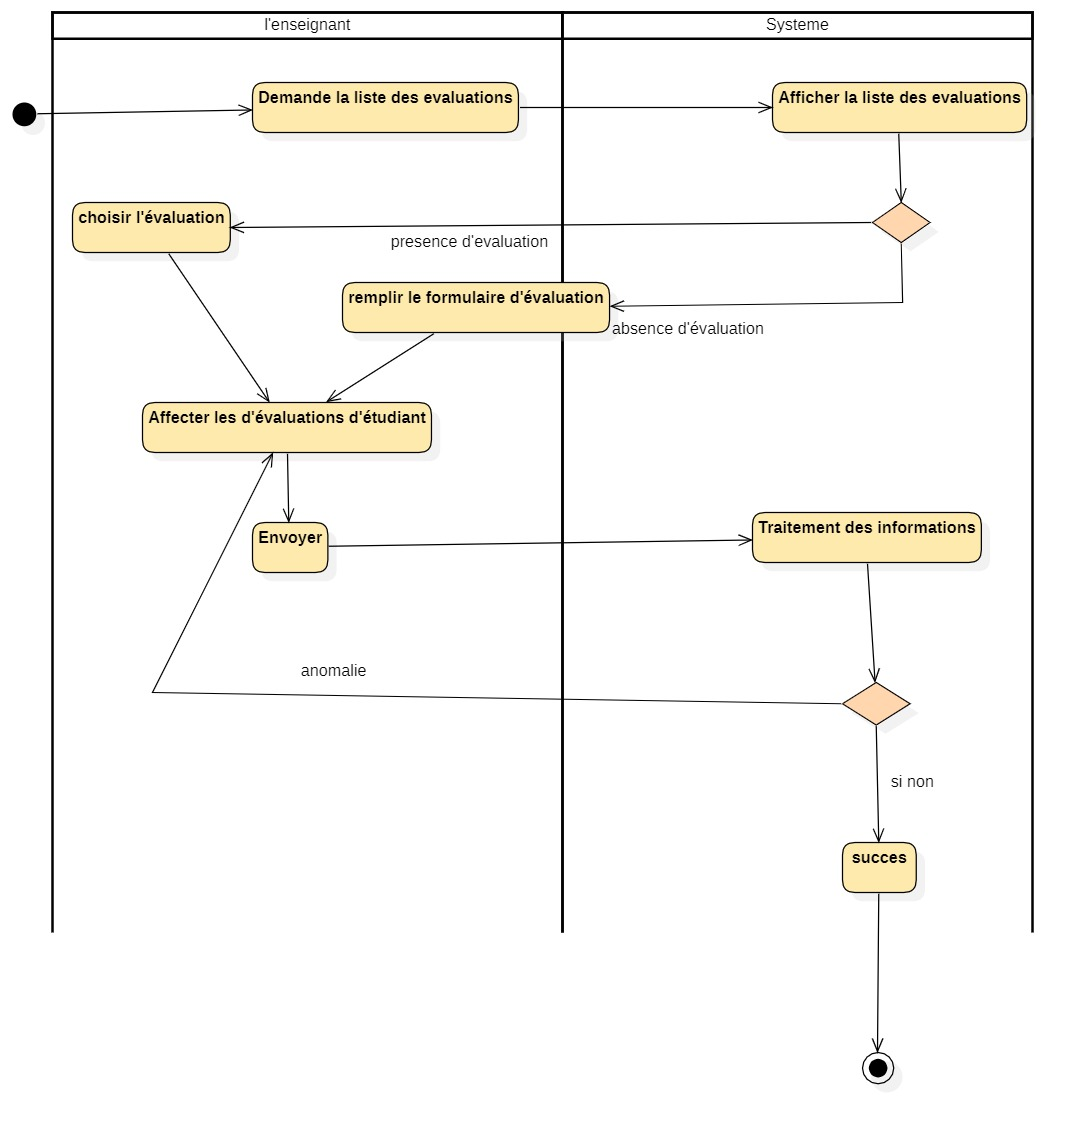
\includegraphics[width=13cm,height=10cm]{Diagrammedactivitésdaffectationdesnotesétudiant.jpg}
	\caption{Diagramme d' activités « d' affectation des notes étudiant » .}
	\label{fig:Diagramme d' activités  d' affectation des notes étudiant   }
\end{figure}
\FloatBarrier

\subsubsubsection{Description du processus de diagramme d’activités «Affecter les notes d’élèves» :}


	\begin{itemize}	
	
	
	
\item[$\star$] L’administration demande la liste des évaluations.
\item[$\star$] Le système affiche la liste des évaluations.
\item[$\star$] En cas d’absence d’évaluation, l’administration doit créer l’évaluation.
\item[$\star$] Si non, l’administration choisit l’évaluation et affecte les notes pour chaque élève.
\item[$\star$] Puis envoyer les notes pour les sauvegarder.
\item[$\star$] Le système traite les informations envoyées.
\item[$\star$] En cas, d’une anomalie l’ajout est annulé.
\item[$\star$] Si non, l’ajout est effectué avec succès.
	
	
	
	
\end{itemize}


\clearpage
\subsubsection{ Interface : Gérer le profil  }
\begin{figure}[ht]
	\centering
	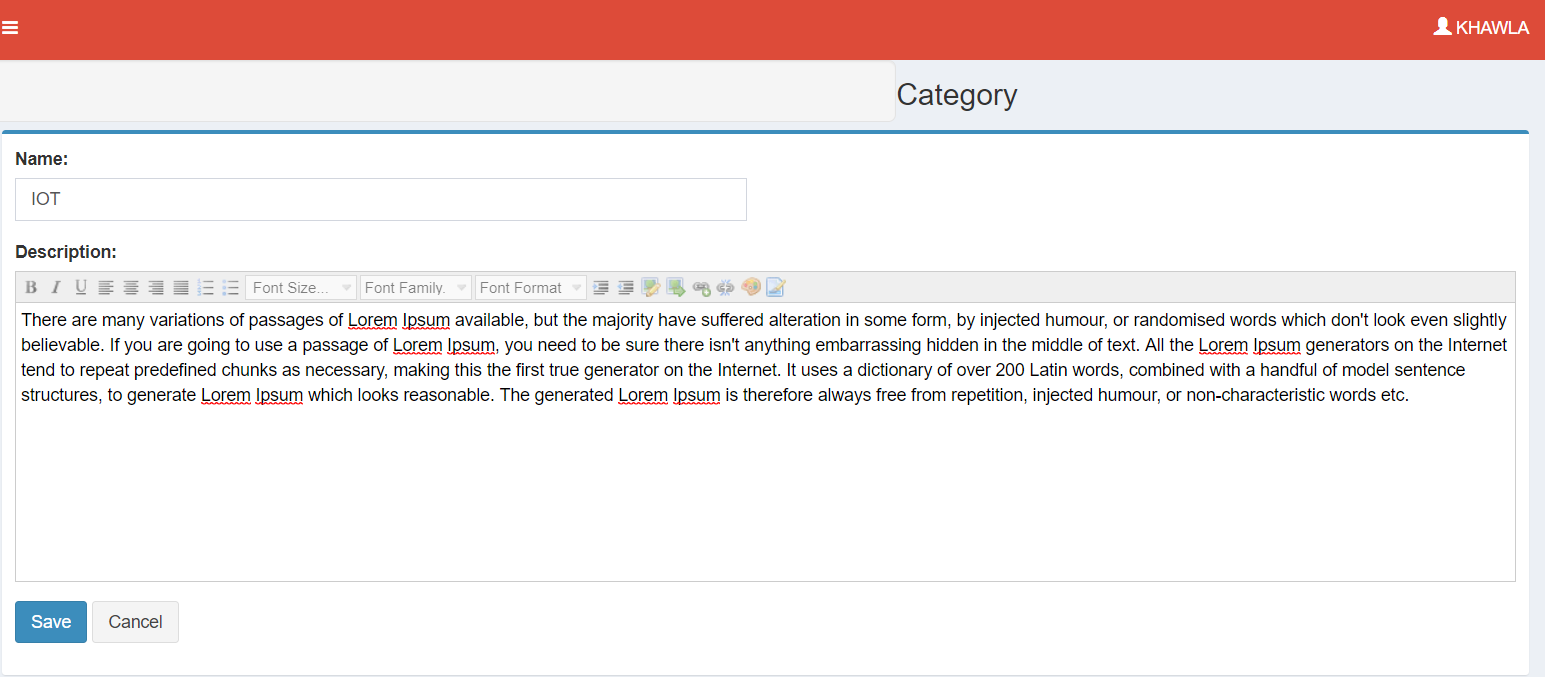
\includegraphics[width=16cm,height=10cm]{12.png}
	\caption{Diagramme de séque de rôle utilisateur .}
	\label{fig:Diagramme de séon de rôle utilisateur }
\end{figure}
\FloatBarrier
\begin{figure}[ht]
	\centering
	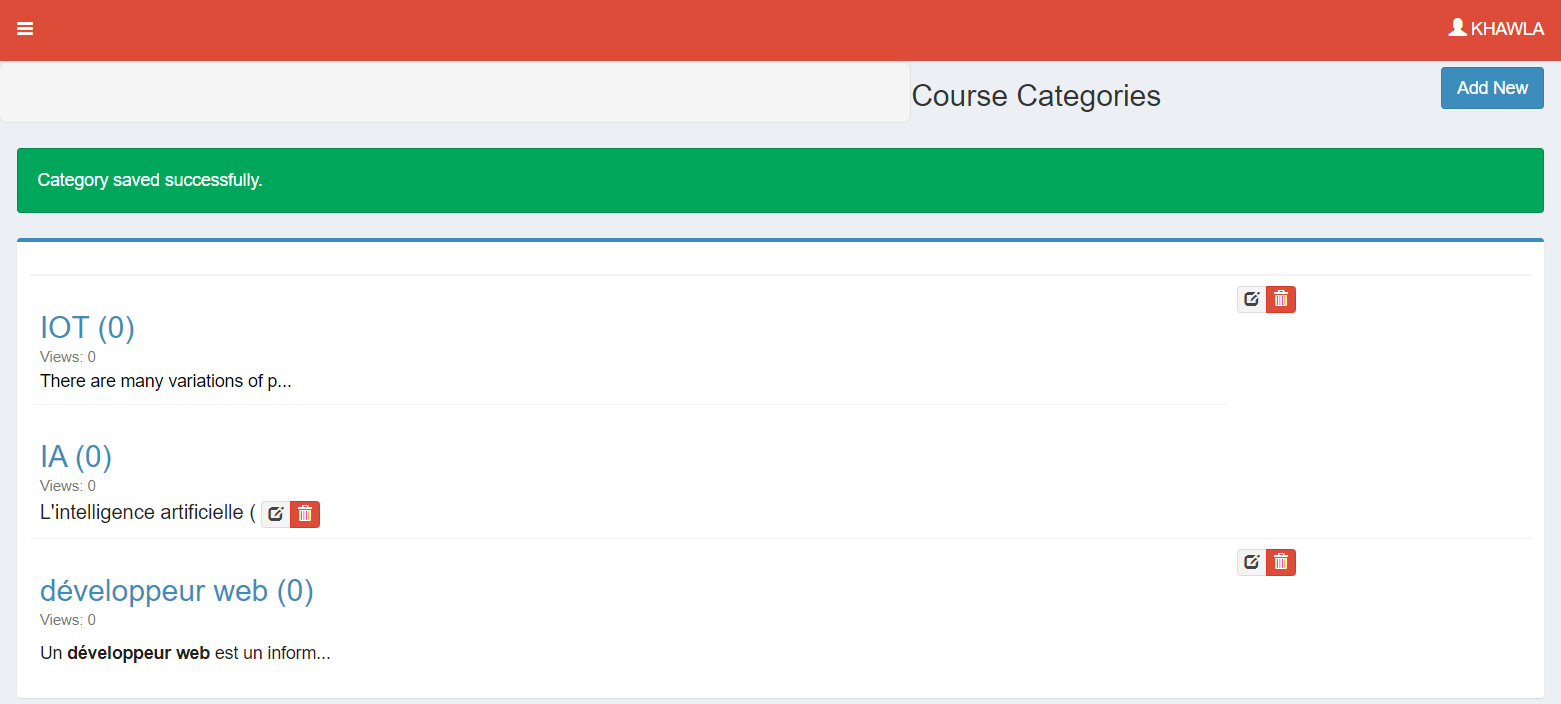
\includegraphics[width=16cm,height=10cm]{13.png}
	\caption{Diagramme de séque e rôle utilisateur .}
	\label{fig:Diagramme d séo rôle utilisateur }
\end{figure}
\FloatBarrier

\begin{figure}[ht]
	\centering
	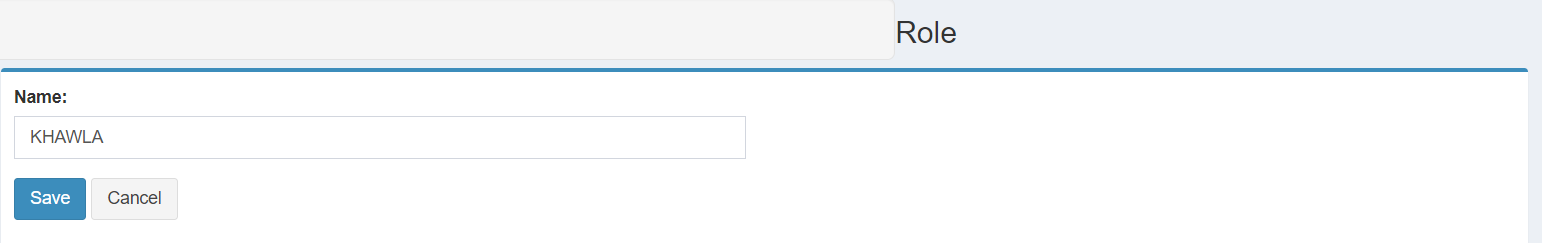
\includegraphics[width=14cm,height=5cm]{5.png}
	\caption{Diagramme de séque e rôle utilisateur .}
	\label{fig:Diagrammde séo rôle utilisateur }
\end{figure}
\FloatBarrier
\begin{figure}[ht]
	\centering
	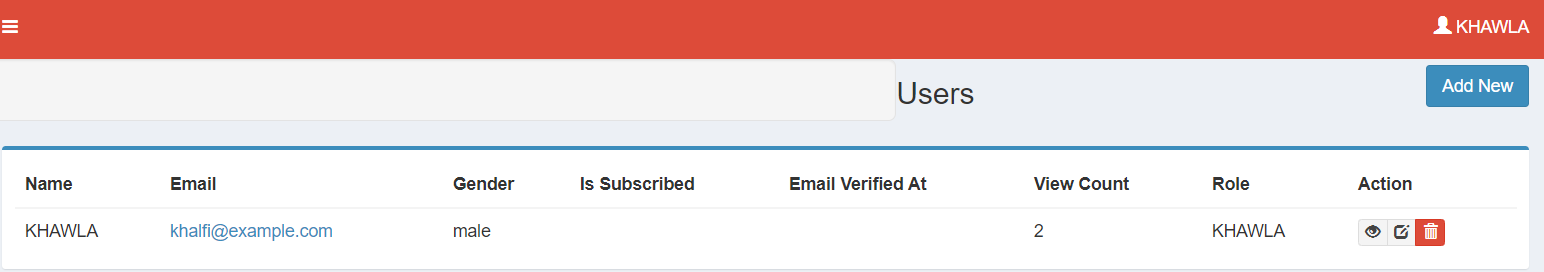
\includegraphics[width=14cm,height=5cm]{9.png}
	\caption{Diagramme de séque e rôe utilisateur .}
	\label{fig:Diagrammde séo rôle utlisateur }
\end{figure}
\FloatBarrier
\begin{figure}[ht]
	\centering
	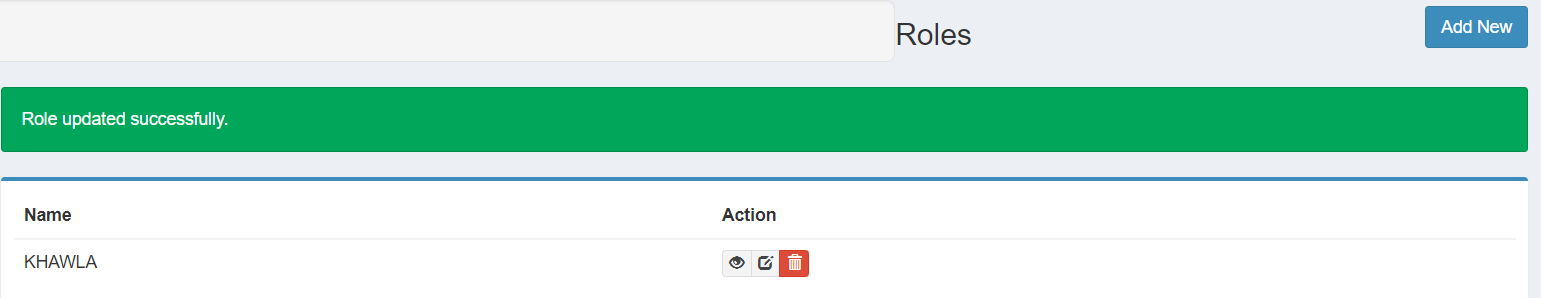
\includegraphics[width=14cm,height=5cm]{6.png}
	\caption{Diagramme de séque e rôe utilisteur .}
	\label{fig:Diagrammde séo rôle utlisater }
\end{figure}
\FloatBarrier
\clearpage

\section{Sprint 3 : Enseignants }
\label{sec:conception}

\begin{fquote}
	Ce premier sprint s’étale sur 18 jours et se décompose en deux items
\end{fquote}
\smallskip
\begin{itemize}[label=$\diamond$]
	\item Gérer les cours 
	
	\item Gérer les  tests
\end{itemize}
\medskip
\medskip
\medskip
\medskip
\medskip
\medskip
\medskip
\medskip
\medskip
\medskip
\medskip
\begin{figure}[ht]
	\centering
	\includegraphics[width=13cm,height=10cm]{Décompositionsprint3enItems.png}
	\caption{Décomposition sprint 3 en Items.}
	\label{fig:Décomposition srint 3 en Items}
\end{figure}
\FloatBarrier
\clearpage






\begin{table}[]
	{\Large\color{cyan} Le backlog du sprint 3 est le suivant :}\\
	
	\begin{tabular}{|l|l|l|l|}
		\hline 
		\rowcolor{-blue!20!red}{Item}                         & \textbf{User Story}                                                   & \textbf{Description}                                                                                              & \textbf{Priorité} \\ \hline
		\textbf{s'inscrire}                    & s'inscrire                                                            & En tant qu'utilisateur, je peux m'inscrire                                                                        & 1    \\ \hline
		\textbf{s'authentifier}                & s'authentifier                                                        & \begin{tabular}[c]{@{}l@{}}En tant qu'utilisateur, je dois m'identifier \\ pour acceder a mon espace\end{tabular} & 2                 \\ \hline
		\multirow{4}{*}{\textbf{gérer profil}} & \begin{tabular}[c]{@{}l@{}}Consulter\\ profil\end{tabular}            & \begin{tabular}[c]{@{}l@{}}En tant qu'utilisateur je peux consulter mon \\ profil\end{tabular}                    & 3                 \\ \cline{2-4} 
		& Modifier profil                                                       & \begin{tabular}[c]{@{}l@{}}En tant qu'utilisateur je peux modifier mon \\ profil\end{tabular}                     &                   \\ \cline{2-4} 
		& \begin{tabular}[c]{@{}l@{}}Modifier\\ image de \\ profil\end{tabular} & \begin{tabular}[c]{@{}l@{}}En tant qu'utilisatuer je peux uploader modifier\\ une image de profil\end{tabular}    &                   \\ \cline{2-4} 
		& Désactiver profil                                                     & \begin{tabular}[c]{@{}l@{}}En tant qu'utilisateur je peux désactiver mon\\ profil\end{tabular}                    &                   \\ \hline
		
		\textbf{s'inscrire}                    & s'inscrire                                                            & En tant qu'utilisateur, je peux m'inscrire                                                                        & 1    \\ \hline
	\end{tabular}
	
	
	\caption{Tables Backlog du sprint 3}
	\label{Tables Backlog du sprint 3}
\end{table}
% \section{end_tableau}










\begin{table}[h]
	{\Large\color{cyan} les user stories de sprint 3:}\\
	
	\begin{center}
		\begin{tabular}{>{\begin{bf} } c <{\end{bf}}ccc}
			
			\rowcolor{-blue!20!red}ID U.S & \begin{bf}User Story \end{bf}  & \\
			
			1 & En tant qu’utilisateur, je dois m’authentifier pour accéder à mon espace \\
			& En tant qu’utilisateur, je  m’authentifier pour accéder à mon espace entifier accéder
			\\
			& \\
			7 & En tant qu’utilisateur, je dois m’authentifier pour accéder à mon espace \\
			
			
		\end{tabular}
	\end{center}
	\caption{Tables  "les user stories de sprint 3"}
	\label{les user stories de sprint 3}
\end{table}


\clearpage

\clearpage

\subsection{item 1 : Gérer les cours}

\subsubsection{Diagramme de cas d’utilisation  détaillé «administrer du site de téléformation» }

\begin{figure}[ht]
	\centering
	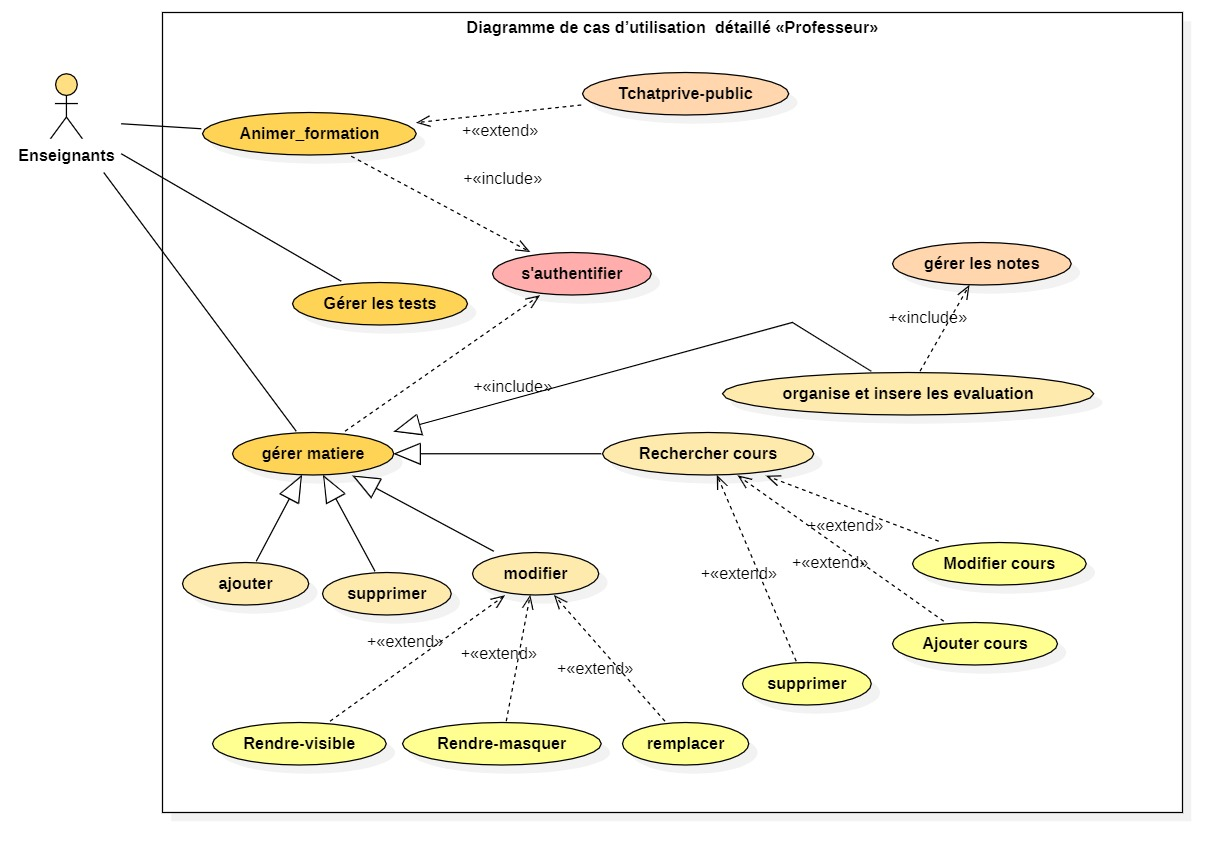
\includegraphics[width=13cm,height=10cm]{DiagrammedecasutilisationdétailléProfesseur.jpg}
	\caption{Diagramme de cas d' utilisation  détaillé «Professeur» .}
	\label{fig:Diagramme de cas d' utilisation  détaillé Professeur  }
\end{figure}
\FloatBarrier

\subsubsubsection{Description détaillée des cas d’utilisations}
\subsubsection{Diagramme des cas d' utilisation  Gérer les cours }
\begin{figure}[ht]
	\centering
	\includegraphics[width=13cm,height=10cm]{CasutilisationGérerlescours.jpg}
	\caption{Diagramme des cas d' utilisation « Gérer les cours » .}
	\label{fig:Diagramme des cas d' utilisation  Gérer les cours  }
\end{figure}
\FloatBarrier

\subsubsubsection{Description détaillée des cas d’utilisations}

\begin{itemize}
	\item[$\bullet$] \textbf{Cas d’utilisation Gérer les cours :}
	\medskip
	\begin{itemize}
		\item \textit{\textbf{Objectif :}}  permet à l’acteur d’ajouter, d’annuler et modifier un cours.
		
		\item \textit{\textbf{Acteur :}} Enseignants
		
		\item \textit{\textbf{Pré-condition :}} L‘acteur doit être connecté.
		\item \textit{\textbf{Scénario nominal   :}}
		\begin{enumerate}
			\item  Le système affiche deux méthodes d’ajout d’un cours.\\
			<méthode1: Créer un cours> 
			\item L’acteur saisit le contenu du cours 
		\end{enumerate}
		<méthode2: téléverser un cours>
		\begin{enumerate}
			\item   L’acteur téléverse le cours.  
			\item  L’acteur configure les droits d’accès à son cour.
			\item  L’acteur enregistre le cours dans la base de données de la plateforme.
		\end{enumerate}
	\end{itemize}
\end{itemize}	
\bigskip



\subsubsection{diagramme de séquences }
\begin{figure}[ht]
	\centering
	\includegraphics[width=13cm,height=10cm]{DiagrammedeséquenceGererlescours.jpg}
	\caption{Diagramme de séquence "Gerer les cours" .}
	\label{fig:Diagramme de séquence "Gerer les cours"  }
\end{figure}
\FloatBarrier

\subsubsubsection{Description :Diagramme de séquence "Gerer les cours"}
Aprés introduire le login et mot de passe l’enseignant peut gérer le cours (Modifier, Ajouter,
Supprimer) Cours, sinon il affiche un message "cours est in trouvée"


\subsubsection{diagramme de séquences }
\begin{figure}[ht]
	\centering
	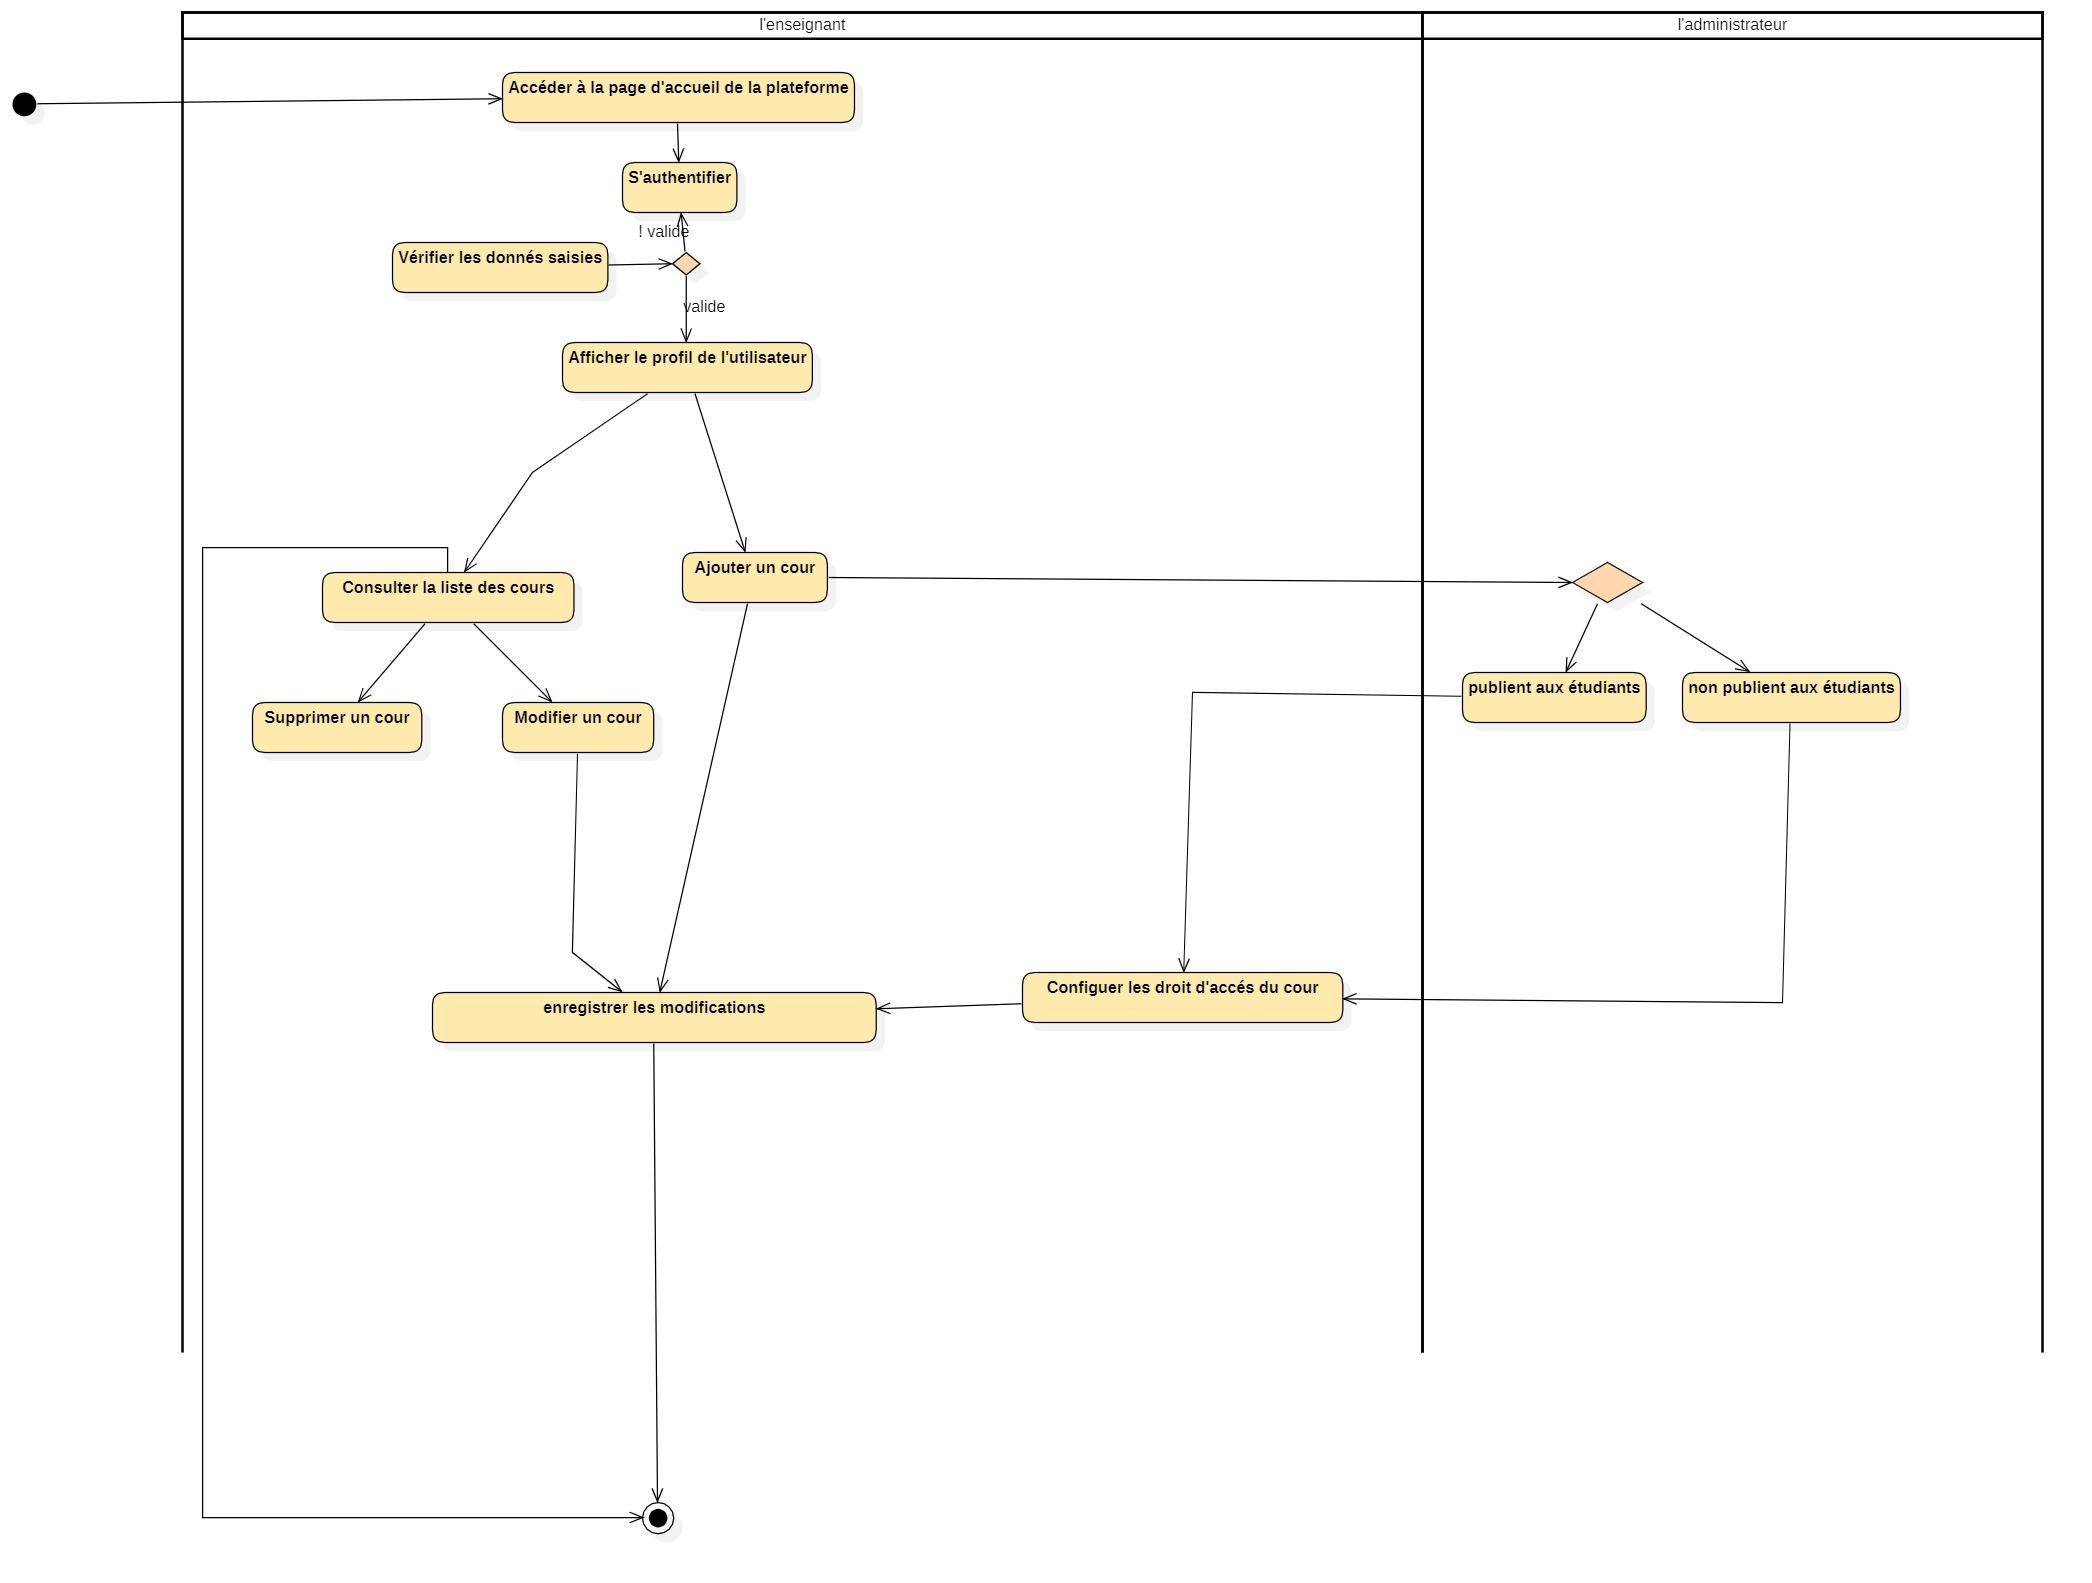
\includegraphics[width=13cm,height=10cm]{DiagrammeactivitésGérerlescou.jpg}
	\caption{Diagramme d' activités « Gérer les cours » .}
	\label{fig:Diagramme d' activités  Gérer les cours  }
\end{figure}
\FloatBarrier

\subsubsubsection{Description détaillée des cas d’utilisations}
La figure ci-dessus illustre le déroulement séquentiel de la gestion des cours accomplis par un Enseignant.\\
Après avoir s’authentifié, un Enseignant peut ajouter, modifier ou supprimer un cours.\\
Au cas d’ajout ou de modification du cours, le tuteur doit ajouter cet évènement  partagé pour informer les apprenants du changement.






\subsubsection{diagramme de séquences }
\begin{figure}[ht]
	\centering
	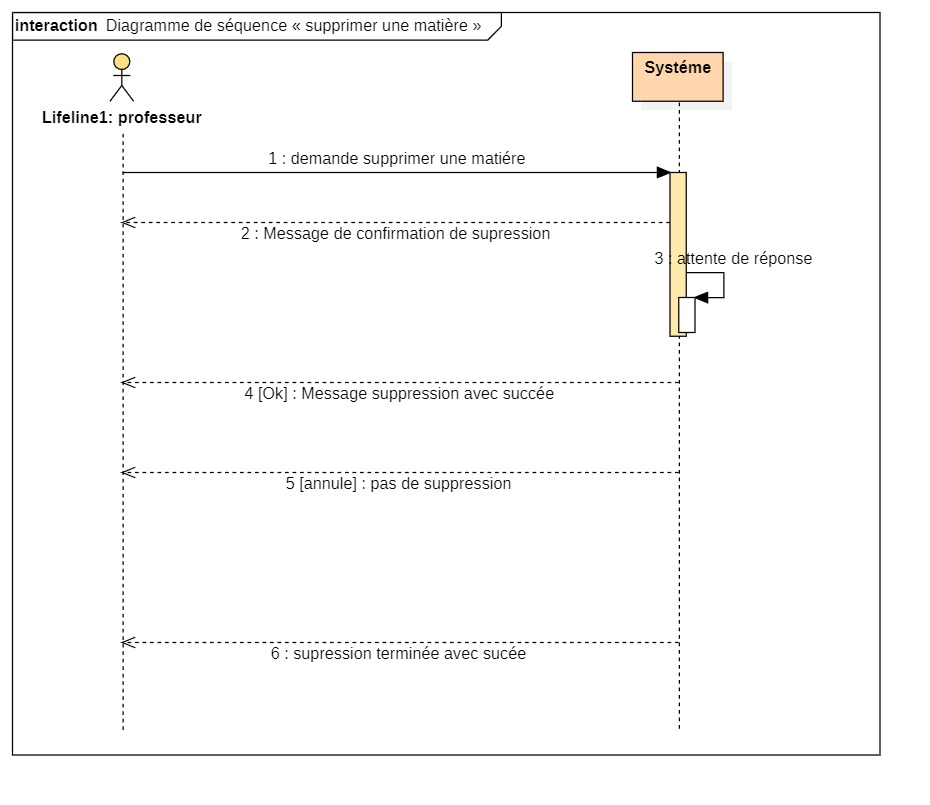
\includegraphics[width=13cm,height=10cm]{Diagrammedeséquencesupprimerunematière.jpg}
	\caption{ Diagramme de séquence « supprimer une matière » .}
	\label{fig: Diagramme de séquence  supprimer une matière   }
\end{figure}
\FloatBarrier

\subsubsubsection{Description détaillée des cas d’utilisations}
















\clearpage
\subsection{item 2 : Gérer les  tests}

\subsubsection{diagramme de séquences }
\begin{figure}[ht]
	\centering
	\includegraphics[width=13cm,height=10cm]{CasdutilisationGérerlestestslesexamens.jpg}
	\caption{Diagramme de Cas d' utilisation « Gérer les tests / les examens » .}
	\label{fig:Diagramme de Cas d' utilisation  Gérer les tests / les examens  }
\end{figure}
\FloatBarrier

\subsubsubsection{Description détaillée des cas d’utilisations}
\begin{itemize}
	\item[$\bullet$] \textbf{Cas d’utilisation Gérer les utilisateurs :} 
	\medskip
	\begin{itemize}
		\item \textit{\textbf{Objectif :}} permet à l’acteur d’ajouter, d’annuler et modifier un test.
		\item \textit{\textbf{Acteur :}} Enseignants
		
		\item \textit{\textbf{Pré-condition  :}} L‘acteur doit être connecté.
		\item \textit{\textbf{Post-conditions   :}}
		\item \textit{\textbf{Scénario nominal :}}
		\begin{enumerate} 
			\item  L’acteur saisit les questions en indiquant la vraie réponse et en précisant un barème. 
			\item    L’acteur configure les droits d’accès au test. 
			\item   L’acteur enregistre le test dans la base de données .  
			\item L’acteur ajoute le test au calendrier partagée et notifie les apprenants de l’ajout du test .
		\end{enumerate}
	\end{itemize}
\end{itemize}	
\bigskip
\subsubsection{diagramme de séquences }
\begin{figure}[ht]
	\centering
	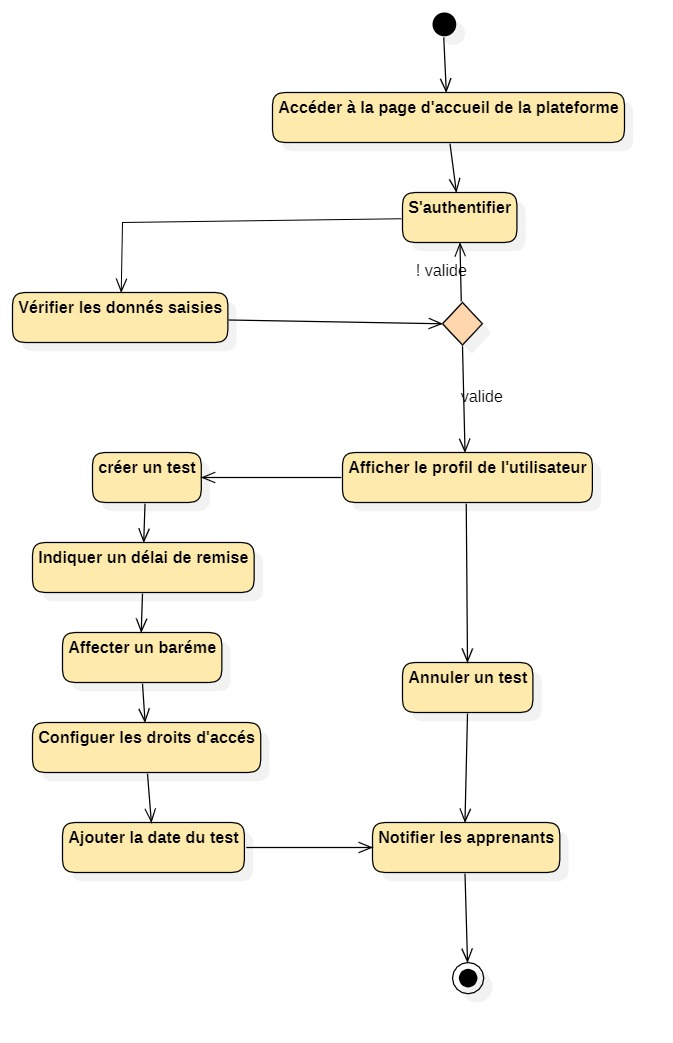
\includegraphics[width=13cm,height=10cm]{DiagrammeactivitésGérerlestestslesexamens.jpg}
	\caption{Diagramme d' activités « Gérer les tests / les examens » .}
	\label{fig:Diagramme d' activités  Gérer les tests / les examens }
\end{figure}
\FloatBarrier
\subsubsubsection{Description détaillée des cas d’utilisations}

La figure ci-dessus illustre le déroulement séquentiel de la gestion des devoirs accomplis par un
Enseignants.\\
Après l’authentification, un Enseignants peut ajouter ou annuler un devoir. Au cas d’ajout, il faut lui
indiquer un délai de remise, lui affecter un barème et lui configurer les droits d’accès.\\
Finalement, et c’est le cas d’annulation aussi, le tuteur doit ajouter l’évènement partagé pour informer l’apprenant du changement .
\clearpage
\subsubsection{ Interface : Gérer le profil  }
\begin{figure}[ht]
	\centering
	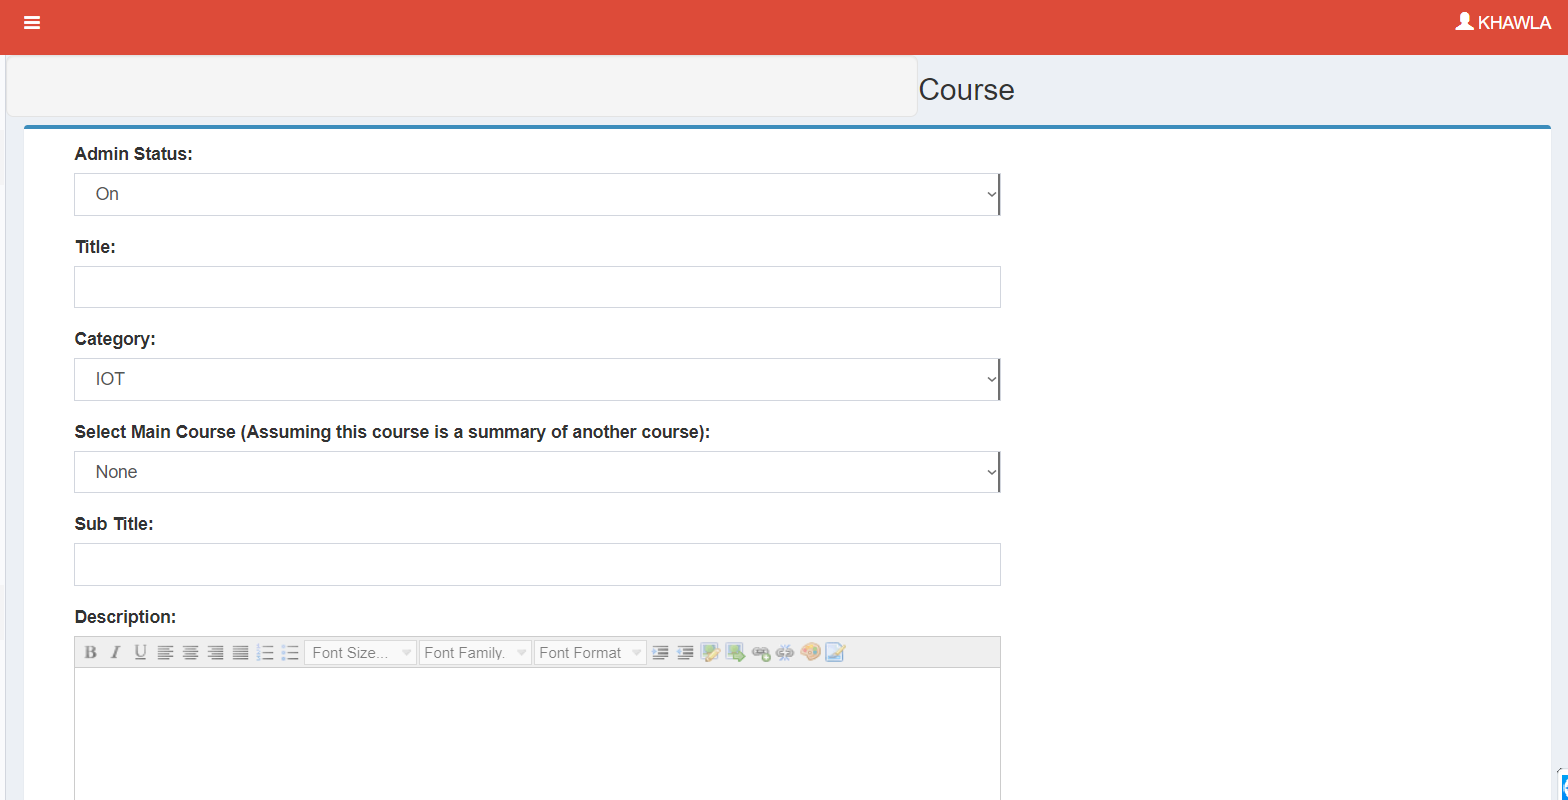
\includegraphics[width=16cm,height=10cm]{14.png}
	\caption{Diagramme de séque de rôle utilisateur .}
	\label{fig:Diagramme de séon de rôle utilisateur }
\end{figure}
\FloatBarrier
\begin{figure}[ht]
	\centering
	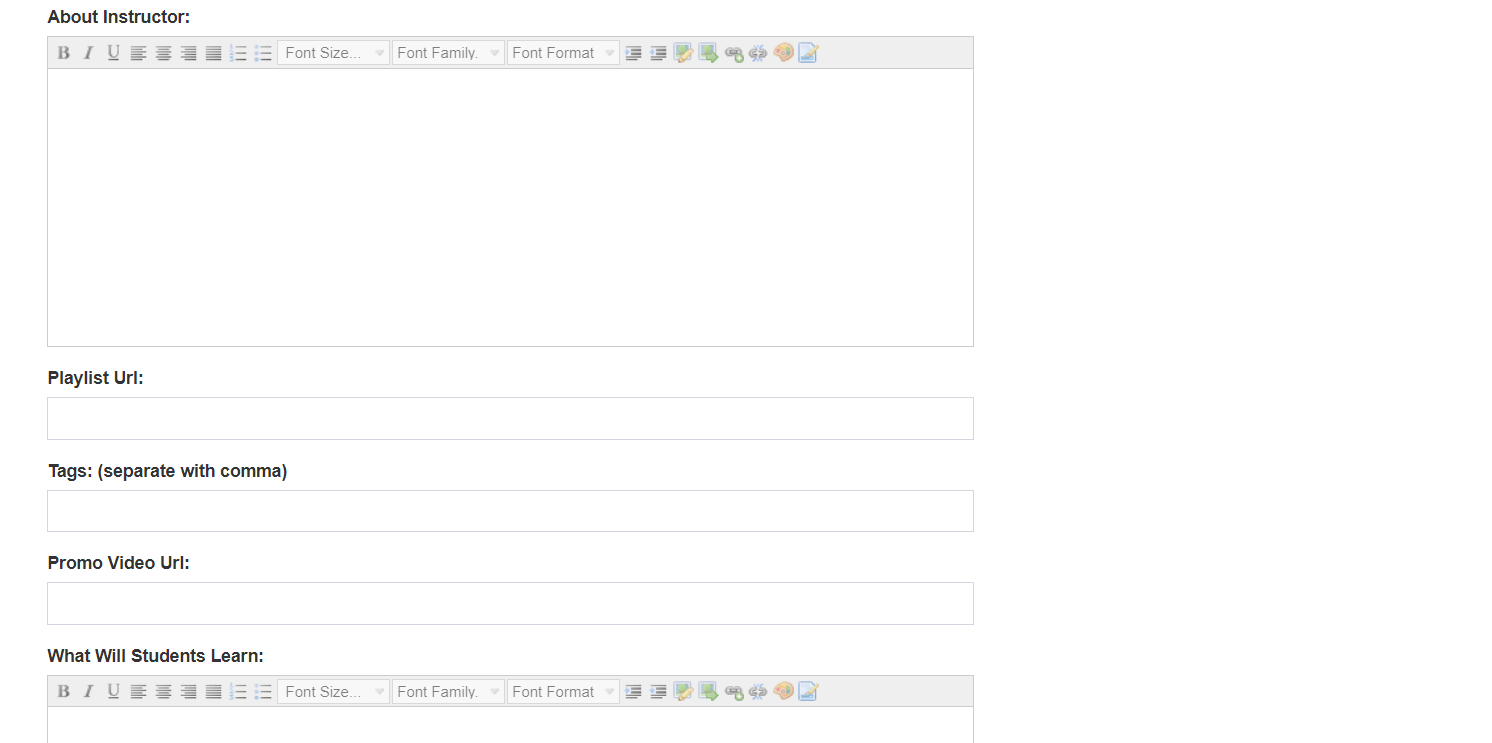
\includegraphics[width=17cm,height=9cm]{15.png}
	\caption{Diagramme de séque de rôle utilisateur .}
	\label{fig:Diagramme de séon de rôle utilisateur }
\end{figure}
\FloatBarrier
\begin{figure}[ht]
	\centering
	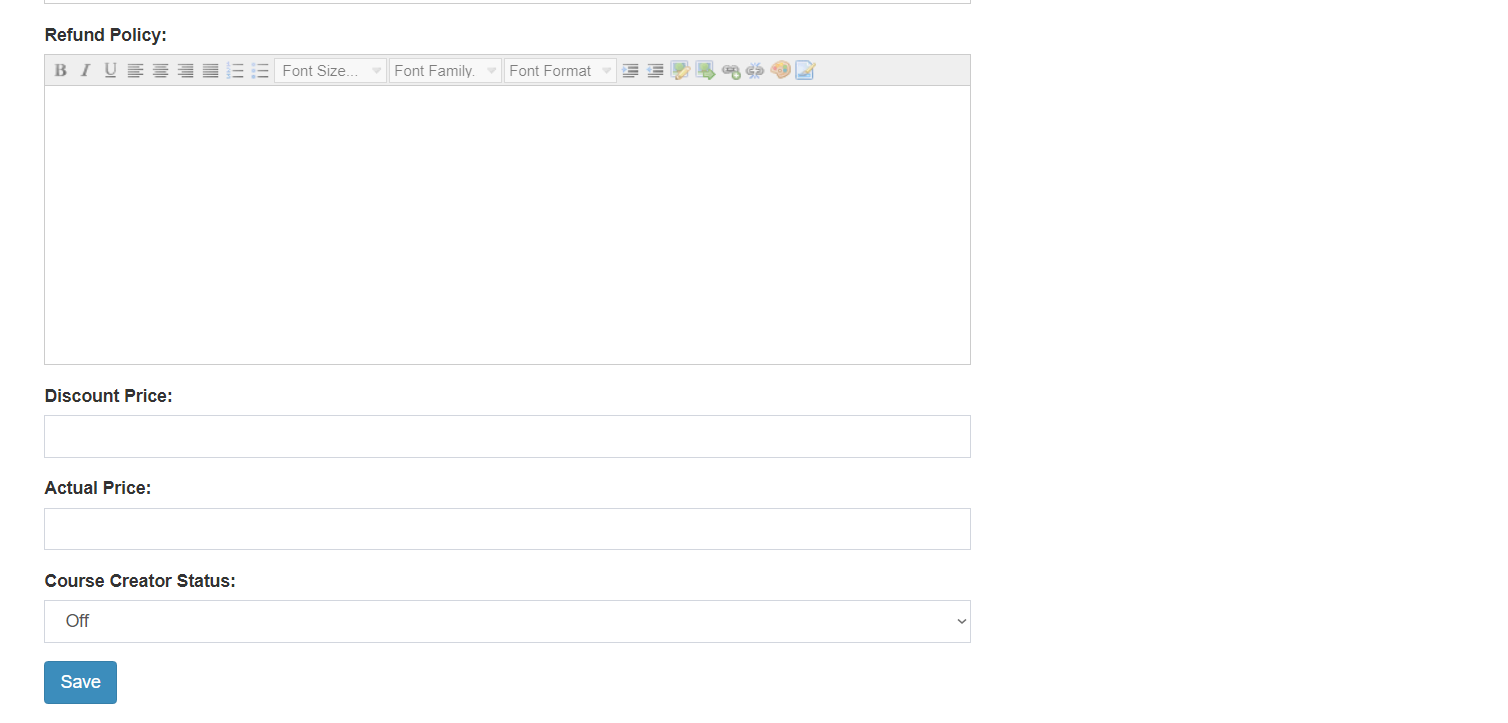
\includegraphics[width=17cm,height=9cm]{16.png}
	\caption{Diagramme de séque de rôle utilisateur .}
	\label{fig:Diagramme de séon de rôle utilisateur }
\end{figure}
\FloatBarrier
\begin{figure}[ht]
	\centering
	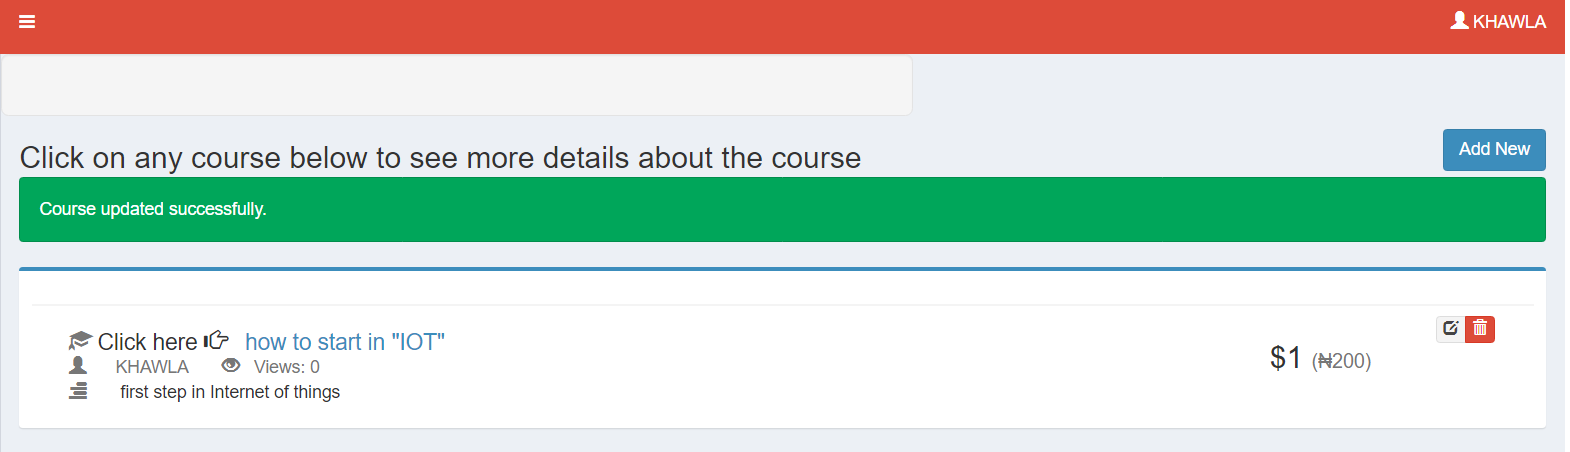
\includegraphics[width=16cm,height=6cm]{17.png}
	\caption{Diagramme de séque de rôle utilisateur .}
	\label{fig:Diagramme de séon de rôle utilisateur }
\end{figure}
\FloatBarrier
\begin{figure}[ht]
	\centering
	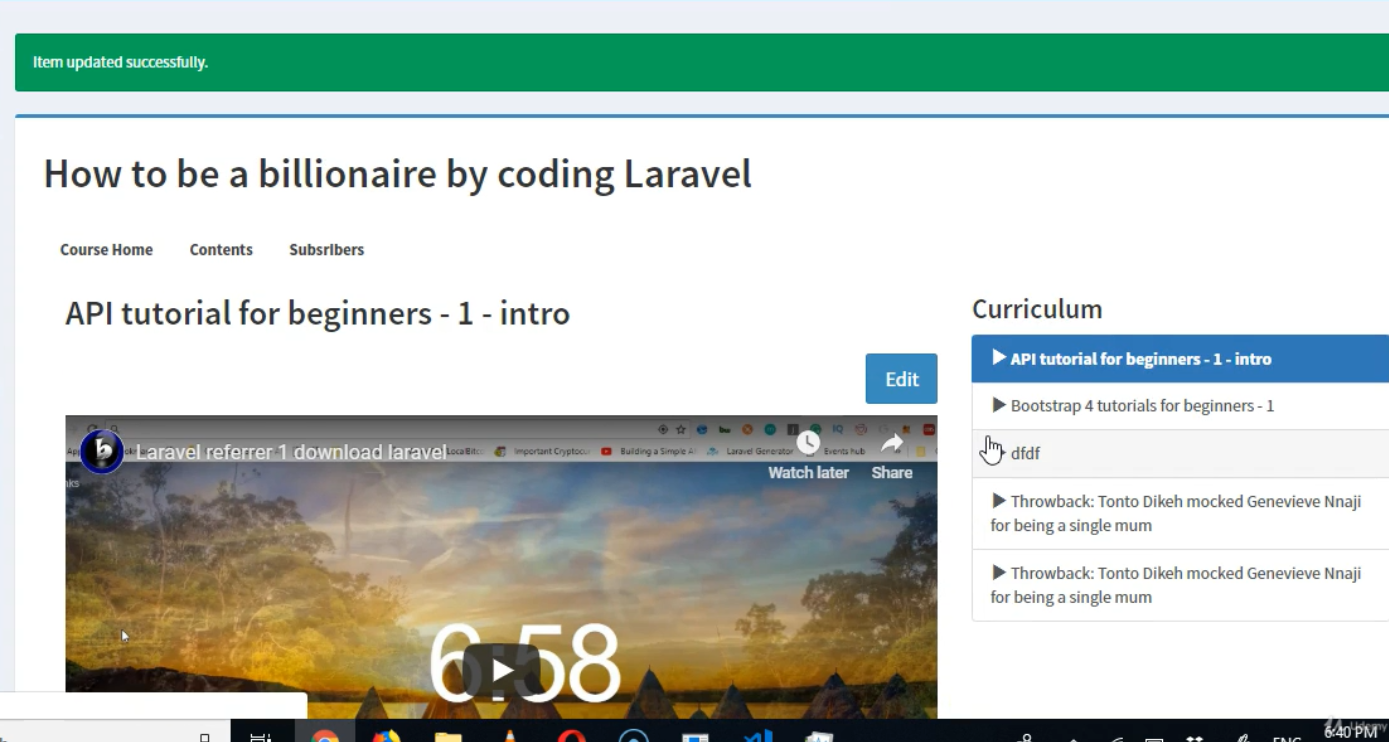
\includegraphics[width=16cm,height=10cm]{Sansrttitgdhgre.png}
	\caption{Diagramme de séque de rôle utilisateur .}
	\label{fig:Diagramme de séon de rôle utilisateur }
\end{figure}
\FloatBarrier
\clearpage
\section{Sprint 4 : Étudiant}
\label{sec:conception}

\begin{fquote}
	Ce premier sprint s’étale sur 21 jours et se décompose en trois items
\end{fquote}
\smallskip
\begin{itemize}[label=$\diamond$]
	\item Consulter les ressources et les liens d'apprentissage
	
	\item Consulter agenda des livrables
	
	\item Passer les examens
	
\end{itemize}
\medskip
\medskip
\medskip
\medskip
\medskip
\medskip
\medskip
\medskip
\medskip
\medskip
\begin{figure}[ht]
	\centering
	\includegraphics[width=13cm,height=10cm]{Décompositionsprint4enItems.png}
	\caption{Décomposition sprint 4 en Items.}
	\label{fig:Démposition sprint 4 en Items}
\end{figure}
\FloatBarrier
\clearpage



\begin{table}[]
	{\Large\color{cyan} Le backlog du sprint 4 est le suivant :}\\
	
	\begin{tabular}{|l|l|l|l|}
		\hline 
		\rowcolor{-blue!20!red}{Item}                         & \textbf{User Story}                                                   & \textbf{Description}                                                                                              & \textbf{Priorité} \\ \hline
		\textbf{s'inscrire}                    & s'inscrire                                                            & En tant qu'utilisateur, je peux m'inscrire                                                                        & 1    \\ \hline
		\textbf{s'authentifier}                & s'authentifier                                                        & \begin{tabular}[c]{@{}l@{}}En tant qu'utilisateur, je dois m'identifier \\ pour acceder a mon espace\end{tabular} & 2                 \\ \hline
		\multirow{4}{*}{\textbf{gérer profil}} & \begin{tabular}[c]{@{}l@{}}Consulter\\ profil\end{tabular}            & \begin{tabular}[c]{@{}l@{}}En tant qu'utilisateur je peux consulter mon \\ profil\end{tabular}                    & 3                 \\ \cline{2-4} 
		& Modifier profil                                                       & \begin{tabular}[c]{@{}l@{}}En tant qu'utilisateur je peux modifier mon \\ profil\end{tabular}                     &                   \\ \cline{2-4} 
		& \begin{tabular}[c]{@{}l@{}}Modifier\\ image de \\ profil\end{tabular} & \begin{tabular}[c]{@{}l@{}}En tant qu'utilisatuer je peux uploader modifier\\ une image de profil\end{tabular}    &                   \\ \cline{2-4} 
		& Désactiver profil                                                     & \begin{tabular}[c]{@{}l@{}}En tant qu'utilisateur je peux désactiver mon\\ profil\end{tabular}                    &                   \\ \hline
		
		\textbf{s'inscrire}                    & s'inscrire                                                            & En tant qu'utilisateur, je peux m'inscrire                                                                        & 1    \\ \hline
	\end{tabular}
	
	
	\caption{Tables Backlog du sprint 4}
	\label{Tables Backlog du sprint 4}
\end{table}
% \section{end_tableau}










\begin{table}[h]
	{\Large \color{cyan} les user stories de sprint 4:}
	
	\begin{center}
		\begin{tabular}{>{\begin{bf} } c <{\end{bf}}ccc}
			
			\rowcolor{-blue!20!red}ID U.S & \begin{bf}User Story \end{bf}  & \\
			
			1 & En tant qu’utilisateur, je dois m’authentifier pour accéder à mon espace \\
			& En tant qu’utilisateur, je  m’authentifier pour accéder à mon espace entifier accéder
			\\
			& \\
			7 & En tant qu’utilisateur, je dois m’authentifier pour accéder à mon espace \\
			
			
		\end{tabular}
	\end{center}
	\caption{Tables  "les user stories de sprint 4"}
	\label{les user stories de sprint 4}
\end{table}



\clearpage
\clearpage
\subsection{item 1 : Consulter les ressources et les liens d'apprentissage}
\subsubsection{Diagramme de cas d’utilisation  détaillé «administrer du site de téléformation» }

\begin{figure}[ht]
	\centering
	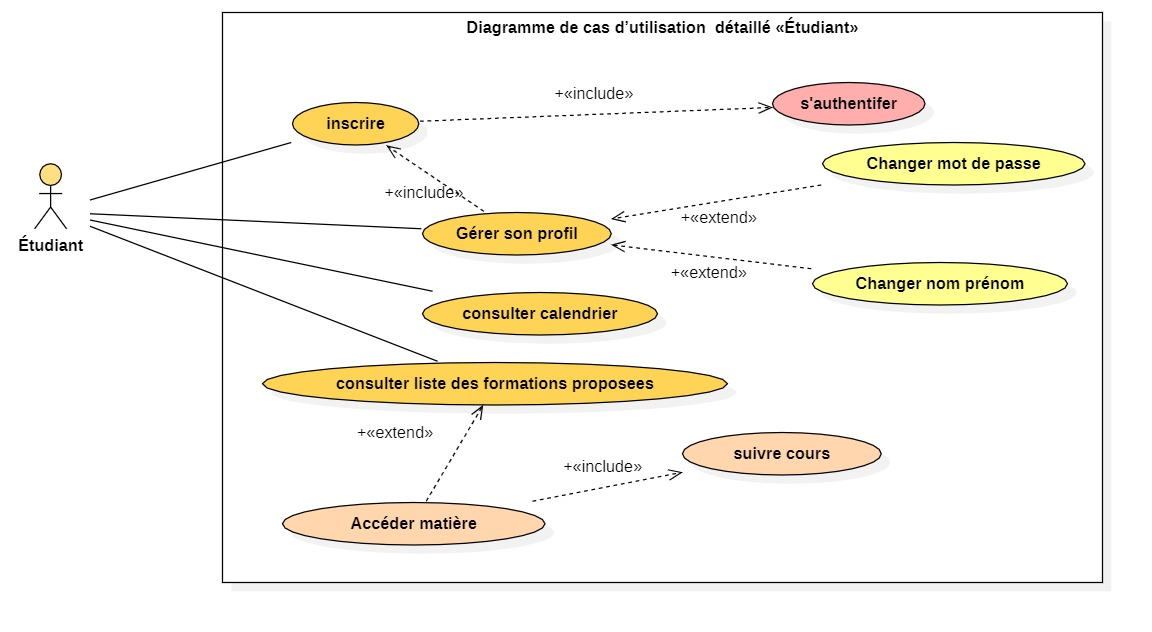
\includegraphics[width=13cm,height=10cm]{DiagrammedecasdutilisationdétailléÉtudiant.jpg}
	\caption{Diagramme de cas d' utilisation  détaillé «Étudiant» .}
	\label{fig:Diagramme de cas d' utilisation  détaillé Étudiant  }
\end{figure}
\FloatBarrier

\subsubsubsection{Description détaillée des cas d’utilisations}





\subsubsection{diagramme de séquences }


\begin{figure}[ht]
	\centering
	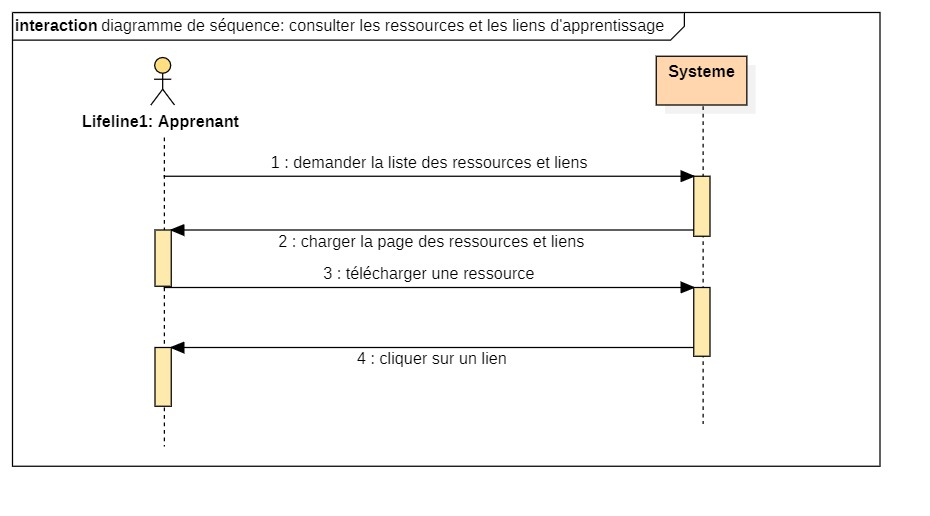
\includegraphics[width=13cm,height=10cm]{dliensapprentissage.jpg}
	\caption{Diagramme de séquence: consulter les ressources et les liens d' apprentissage .}
	\label{fig:diagramme de séquence: consulter les ressources et les liens d' apprentissage }
\end{figure}
\FloatBarrier

\subsubsubsection{Description détaillée des cas d’utilisations}



\clearpage
\subsection{item 2 : Consulter agenda des livrables}
\subsubsection{diagramme de séquences }


\begin{figure}[ht]
	\centering
	\includegraphics[width=13cm,height=10cm]{diagrammedeséquencesconsulteragendadeslivrable.jpg}
	\caption{Diagramme de séquences consulter agenda des livrables .}
	\label{fig:Diagramme de séquences consulter agenda des livrables }
\end{figure}
\FloatBarrier

\subsubsubsection{Description : Diagramme de séquences consulter agenda des livrables}
Ce diagramme de séquence illustre l’interaction entre l’apprenant et le système afin de consulter le
calendrier des livrables d’un projet dont il est participant.
\clearpage
\subsection{item 3 : Passer les examens}
\subsubsection{Diagramme de cas d’utilisation }


\begin{figure}[ht]
	\centering
	\includegraphics[width=13cm,height=10cm]{DiagrammedeséquencePasserlesexamens.jpg}
	\caption{Diagramme de séquence " Passer les examens" .}
	\label{fig:Diagramme de séquence " Passer les examens" }
\end{figure}
\FloatBarrier

\subsubsubsection{Description :Diagramme de séquence " Passer les examens"}

l’etudiant peut passer les examens en une durée du temps detérminé , sinon il affiche un
message "examen est in trouvée"

\begin{figure}[ht]
	\centering
	\includegraphics[width=13cm,height=10cm]{Diagrammedactivitédunapprenantsurlespace.jpg}
	\caption{Diagramme d' activité: d' un apprenant sur l' espace .}
	\label{fig:Diagramme d' activité: d' un apprenant sur l' espace }
\end{figure}
\FloatBarrier

\subsubsubsection{Description détaillée des cas d’utilisations}
Ce digramme d’activités décrit les activités d’un apprenant sur l’espace destiné aux projets
afin de garantir l’apprentissage par projet.



\subsubsection{ Interface : Gérer le profil  }

\clearpage
\begin{figure}[ht]
	\centering
	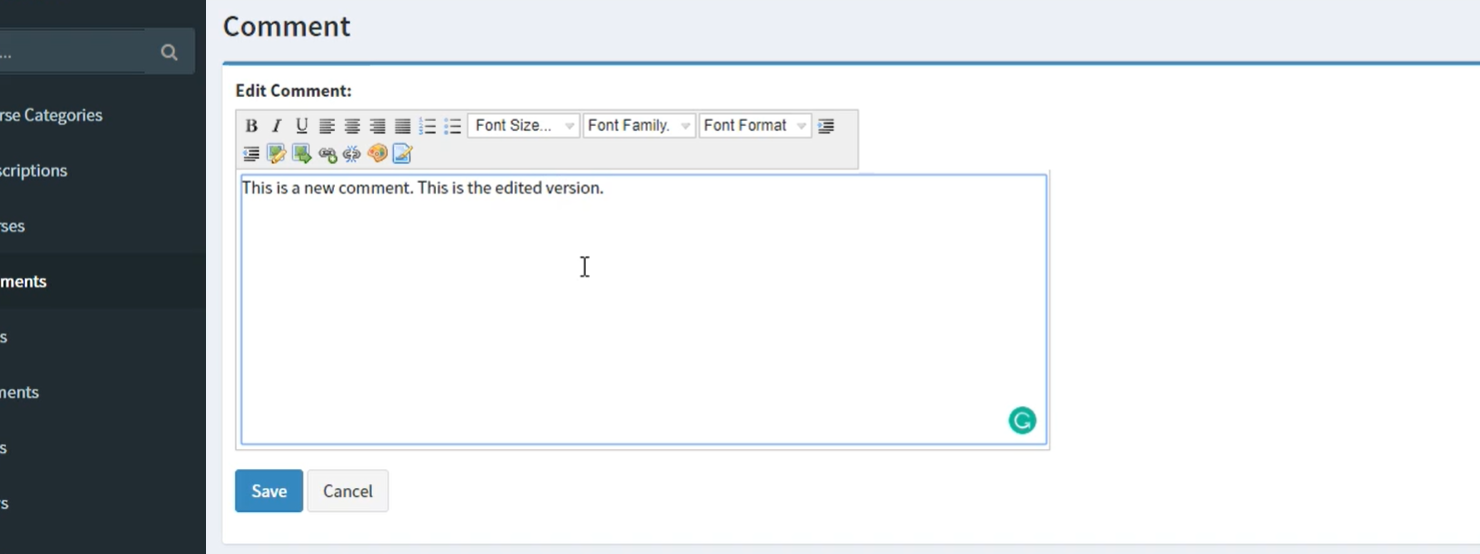
\includegraphics[width=17cm,height=8cm]{Sae.png}
	\caption{Interface : Gérer le profil .}
	\label{fig:Interface : Gérer le profil }
\end{figure}
\FloatBarrier

\begin{figure}[ht]
	\centering
	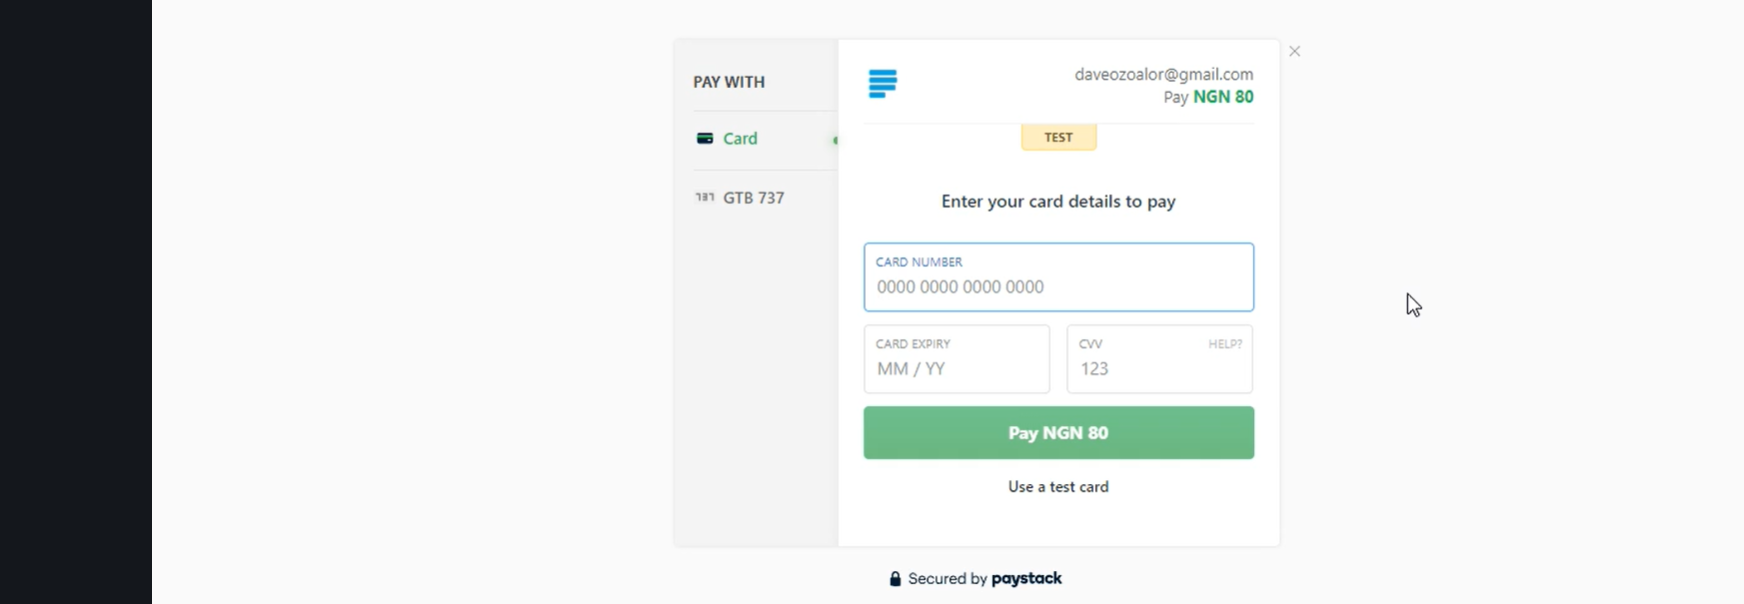
\includegraphics[width=17cm,height=8cm]{Santrmkmkmke.png}
	\caption{Interface : Gérer le profil .}
	\label{fig:Interface : Gérer le profil }
\end{figure}
\FloatBarrier


\begin{figure}[ht]
	\centering
	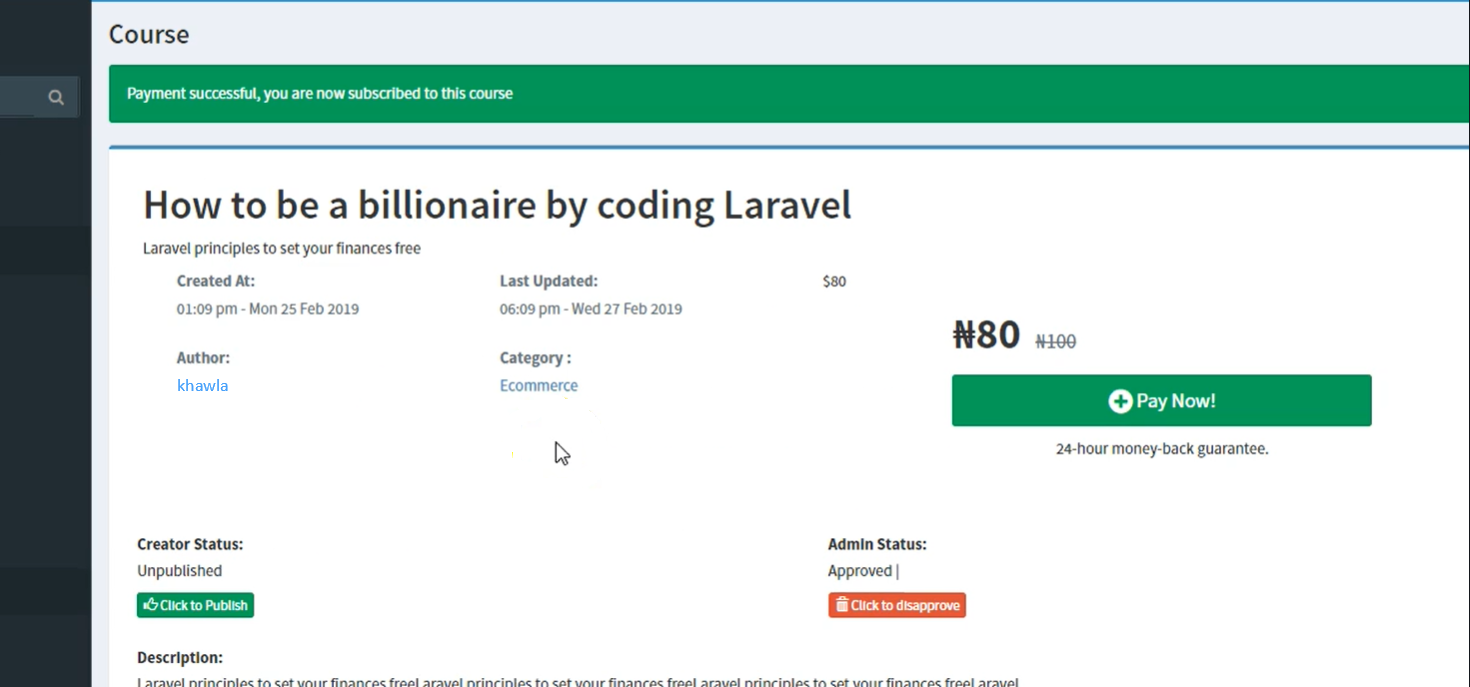
\includegraphics[width=17cm,height=8cm]{Sanstidgsfdghjtre.png}
	\caption{Interface : Gérer le profil .}
	\label{fig:Interface : Gérer le profil }
\end{figure}
\FloatBarrier

\begin{figure}[ht]
	\centering
	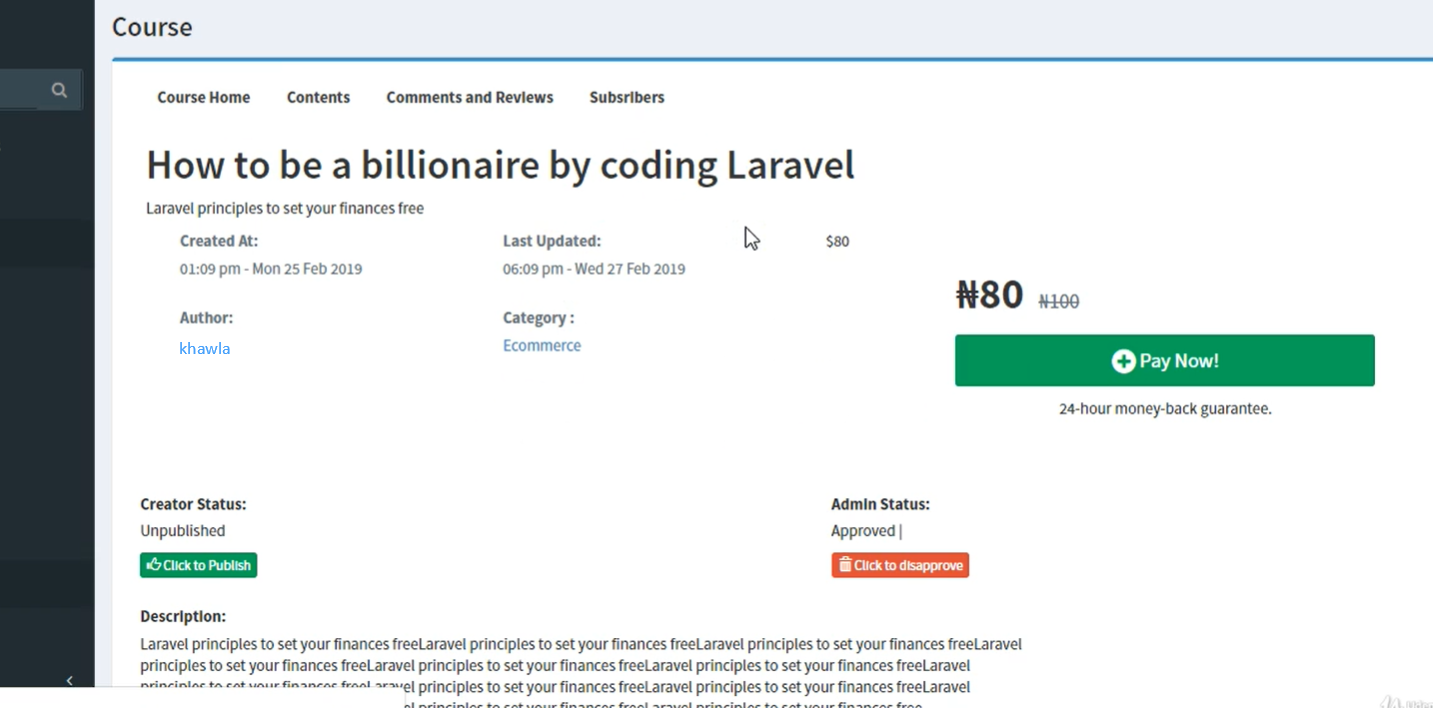
\includegraphics[width=17cm,height=8cm]{Sanstisdfgtre.png}
	\caption{Interface : Gérer le profil .}
	\label{fig:Interface : Gérer le profil }
\end{figure}
\FloatBarrier



\begin{figure}[ht]
	\centering
	\includegraphics[width=17cm,height=8cm]{Sasdfghre.png}
	\caption{Interface : Gérer le profil .}
	\label{fig:Interface : Gérer le profil }
\end{figure}
\FloatBarrier
\clearpage

\section{Conclusion}

Ce chapitre présente une vue conceptuelle de la solution à mettre en place. Il expose les différents diagrammes UML pour mieux comprendre les fonctionnalités offertes et pour mieux représenter la communication entre les différents objets du projet. Le chapitre suivant, présente la partie mise en œuvre de l’application.


